\documentclass[master=cws,masteroption=se,english,oneside,a4paper]{kulemt}
\setup{
	title={A comparative study of cross-platform tools for mobile application development},
  	author={Michiel~Staessen},
  	assessor={},
  	promotor={prof.\,dr.\,ir.\ Erik~Duval},
  	assistant={ir.\ Gonzalo~Parra}
}

% The following \setup may be removed entirely if no filing card is wanted
\setup{
	filingcard,
	translatedtitle="Een vergelijkende studie van cross-platform tools voor het ontwikkelen van mobiele applicaties",
	udc=,
	shortabstract={
		Developing mobile applications (apps) for multiple platforms is an expensive and time consuming process. Therefore, many companies are seeking refuge in Cross-Platform Tools (CPTs) for the development of their apps. In cooperation with CapGemini, this thesis presents a comparison of two such cross-platform tools: Apache Cordova and Motorola Rhodes. Both tools are compared with each other and with native development. The comparison is based on a proof-of-concept application which should work on both smartphones and tablets with respect to both iOS and Android.
	}
}

% Uncomment the next line for generating the cover page
%\setup{coverpageonly}
% Uncomment the next \setup to generate only the first pages (e.g., if you
% are a Word user.
%\setup{frontpagesonly}

% Choose the main text font (e.g., Latin Modern)
\setup{
	font=utopia
}

%% Additional formatting settings
%  Use the chapter and headings styles as well as the ToC formatting
%  as defined in the kulemtx document style
\usepackage{kulemtx}
\headstyles{kulemtman}
\kulemtmanToC

% If you want to include other LaTeX packages, do it here.
\usepackage{url}

% Finally the hyperref package is used for pdf files.
% This can be commented out for printed versions.
\usepackage[pdfusetitle,colorlinks,plainpages=false]{hyperref}

\usepackage[square,numbers]{natbib}
\usepackage{amsmath}
\usepackage{amsfonts}
\usepackage{xfrac}
\usepackage{parskip}
%\usepackage{pstricks}
%\usepackage{pst-node}

% Paragraph definition
\setlength{\parindent}{0pt}
\setlength{\parskip}{2.3ex plus 0.3ex minus 0.3ex}

\newcommand{\npar}{}
\newcommand{\citeGartner}{\cite{Gartner:08Q2, Gartner:08Q3, Gartner:08Q4, Gartner:10Q1, Gartner:10Q2, Gartner:10Q3, Gartner:10Q4, Gartner:11Q1, Gartner:11Q2, Gartner:11Q3, Gartner:11Q4, Gartner:12Q1, Gartner:12Q2, Gartner:12Q3, Gartner:12Q4}}
\newcommand{\citeGartnerTab}{\cite{Gartner:11tab,Gartner:12tab}}
\newcommand{\TODO}[1]{\textcolor{red}{TODO: #1}}

\begin{document}

\begin{preface}
    % dankwoord
\end{preface}

\tableofcontents*

\begin{abstract}
    The \texttt{abstract} environment contains a more extensive overview of
    the work. But it should be limited to one page.
\end{abstract}

% A list of figures and tables is optional
%\listoffigures
%\listoftables

% If you only have a few figures and tables you can use the following instead
%\listoffiguresandtables

% The list of symbols is also optional.
% This list must be created manually, e.g., as follows:
%\chapter{List of Abbreviations and Symbols}
%\section*{Abbreviations}
%\begin{flushleft}
%  \renewcommand{\arraystretch}{1.1}
%  \begin{tabularx}{\textwidth}{@{}p{12mm}X@{}}
%    PoC   & Proof of Concept \\
%    CPT   & Cross-Platform Tool \\
%    PSNR  & Peak Signal-to-Noise ratio \\
%  \end{tabularx}
%\end{flushleft}
%\section*{Symbols}
%\begin{flushleft}
%  \renewcommand{\arraystretch}{1.1}
%  \begin{tabularx}{\textwidth}{@{}p{12mm}X@{}}
%    42    & ``The Answer to the Ultimate Question of Life, the Universe,
%            and Everything'' according to \cite{h2g2} \\
%    $c$   & Speed of light \\
%    $E$   & Energy \\
%    $m$   & Mass \\
%    $\pi$ & The number pi \\
%  \end{tabularx}
%\end{flushleft}

% Now comes the main text
\mainmatter

\chapter{Introduction}
\label{cha:intro}

The mobile industry is without a doubt one of the most vibrant industries at the moment. It is characterized by rapid growth and intense competition which has led to fragmentation. This chapter first presents an overview of the evolution in the mobile device landscape, then explains the problem of fragmentation and how cross-platform tools (CPTs) can help solve this problem and finally, the goals of this thesis are defined.

\section{The mobile device landscape}

Mobile phones have been around since the nineties but ever since the (nearly simultaneous) introduction of the iPhone 3G and the HTC Dream in 2008, smartphones are taking over from traditional cell phones or feature phones. A feature phone (sometimes also called a dumb phone) is a low-end mobile phone, providing only basic telephony and texting capabilities. Smartphones on the other hand are high-end devices that combine the functionality of mobile phones with the functionality of a portable computer. These devices have advanced computing power and often include multiple connectivity options (cellular, Wi-Fi, Bluetooth, NFC, etc.), sensors (GPS, compass, accelerometer, etc.), applications, etc. In the last five years, smartphone sales have grown tremendously. According to quarterly studies by Gartner\footnote{Gartner is an American research and advisory firm, specialized in information technology, \url{http://www.gartner.com}.} \citeGartner, smartphone sales have grown 544\% since the second quarter of 2008 (see \fref{fig:smartphone-sales}). Smartphones are becoming ubiquitous and in some regions like the United States, smartphone penetration\footnote{this is the ratio between smartphones and all mobile phones} has already reached more than 50\% \cite{Nielsen:2012}. 

\begin{figure}[h]
    \centering
    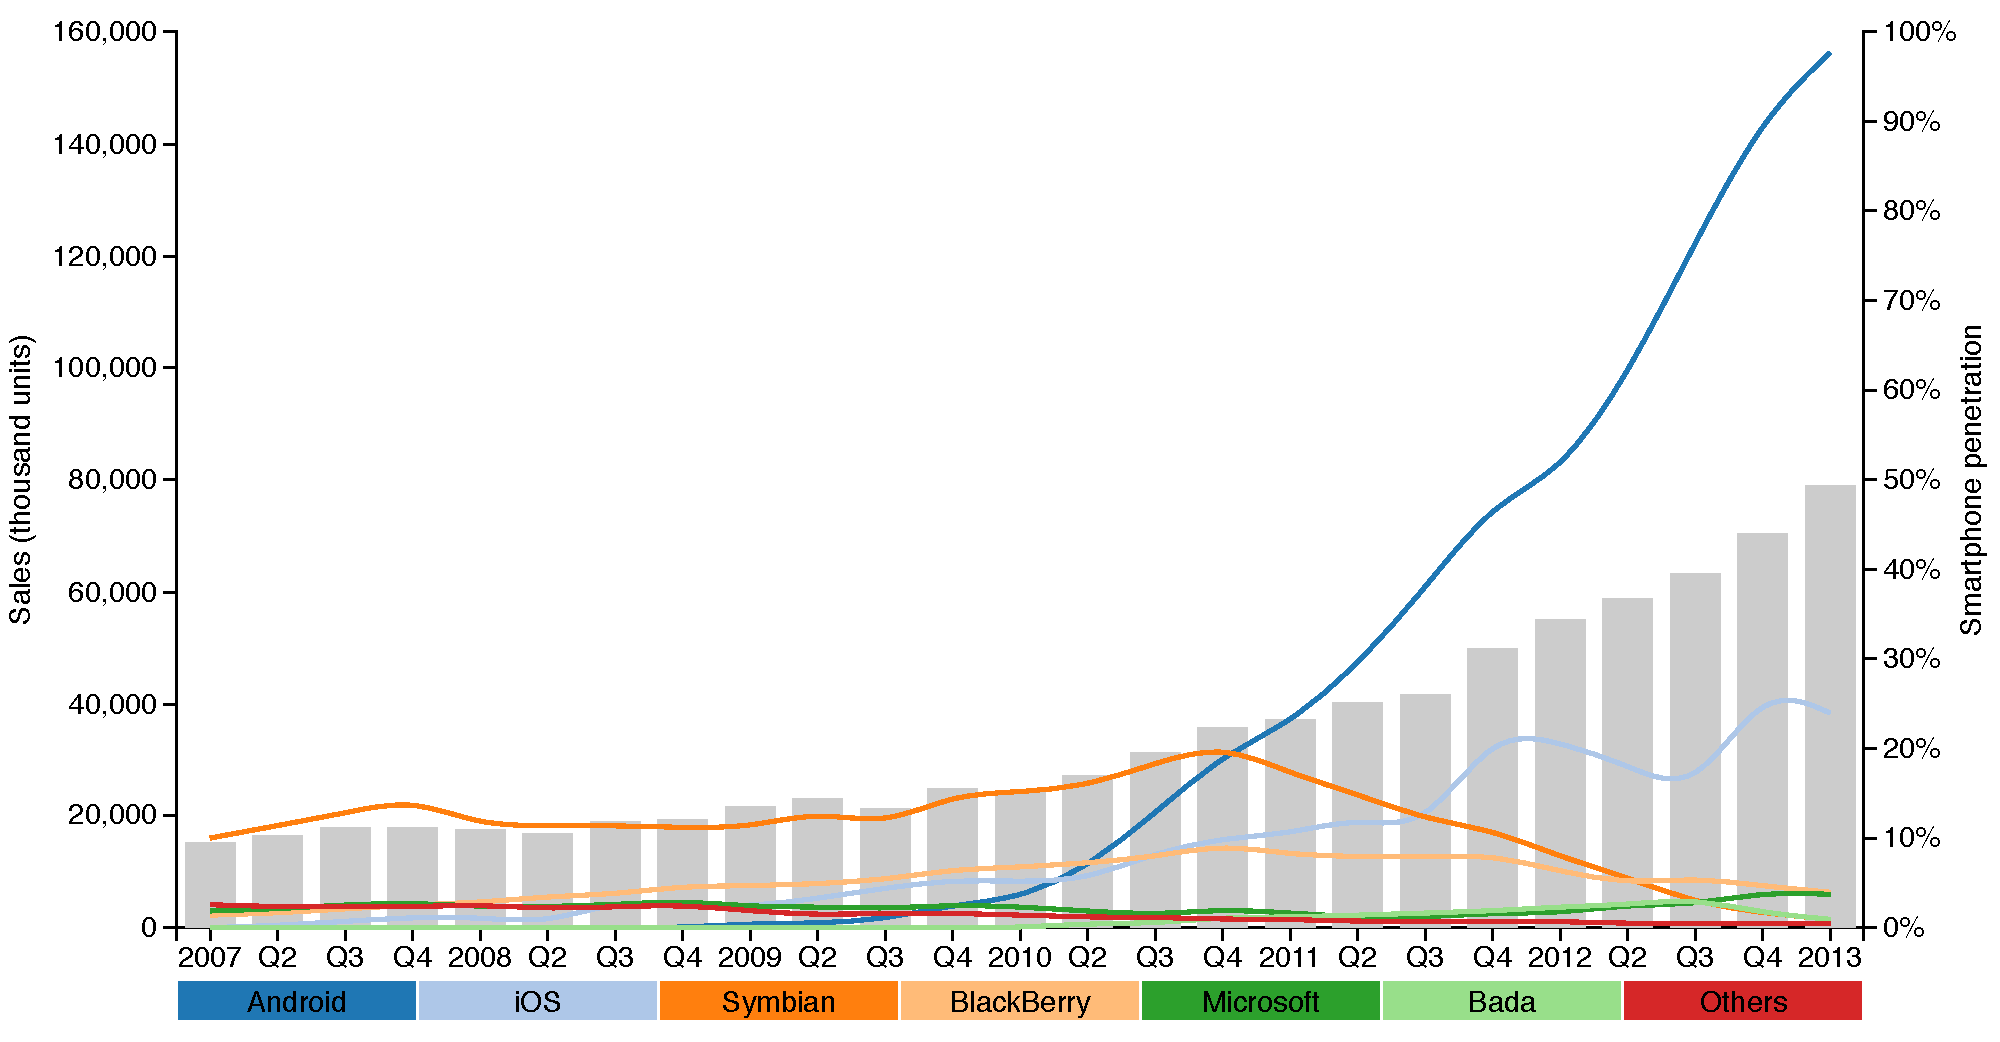
\includegraphics[width=\textwidth]{../resources/figs/smartphone_sales.pdf}
    	\caption{Evolution of worldwide smartphone sales by operating system (lines) and smartphone penetration (bars). Source: Gartner \citeGartner}
    	\label{fig:smartphone-sales}
\end{figure}

Each of these smartphones comes with a mobile operating system which allows owners to run third-party software, typically called applications or apps for short, on their device. These application play an important role as they drive the network effects associated with a certain platform. Applications create additional value for a platform, which attracts new users. Whenever a platform attracts more users, it becomes even more valuable. This vicious circle is called a network effect. Network effects make it hard for new platforms to gain traction which is visible in \fref{fig:smartphone-sales} and \fref{fig:smartphone-share}. Android and iOS are currently dominant (and continue growing) while other platforms are either in decline (like Symbian and Blackberry, formerly RIM) or have a hard time getting traction (like Windows Phone, the successor of Windows Mobile, which already existed before Android and iOS).

\begin{figure}[h]
    \centering
    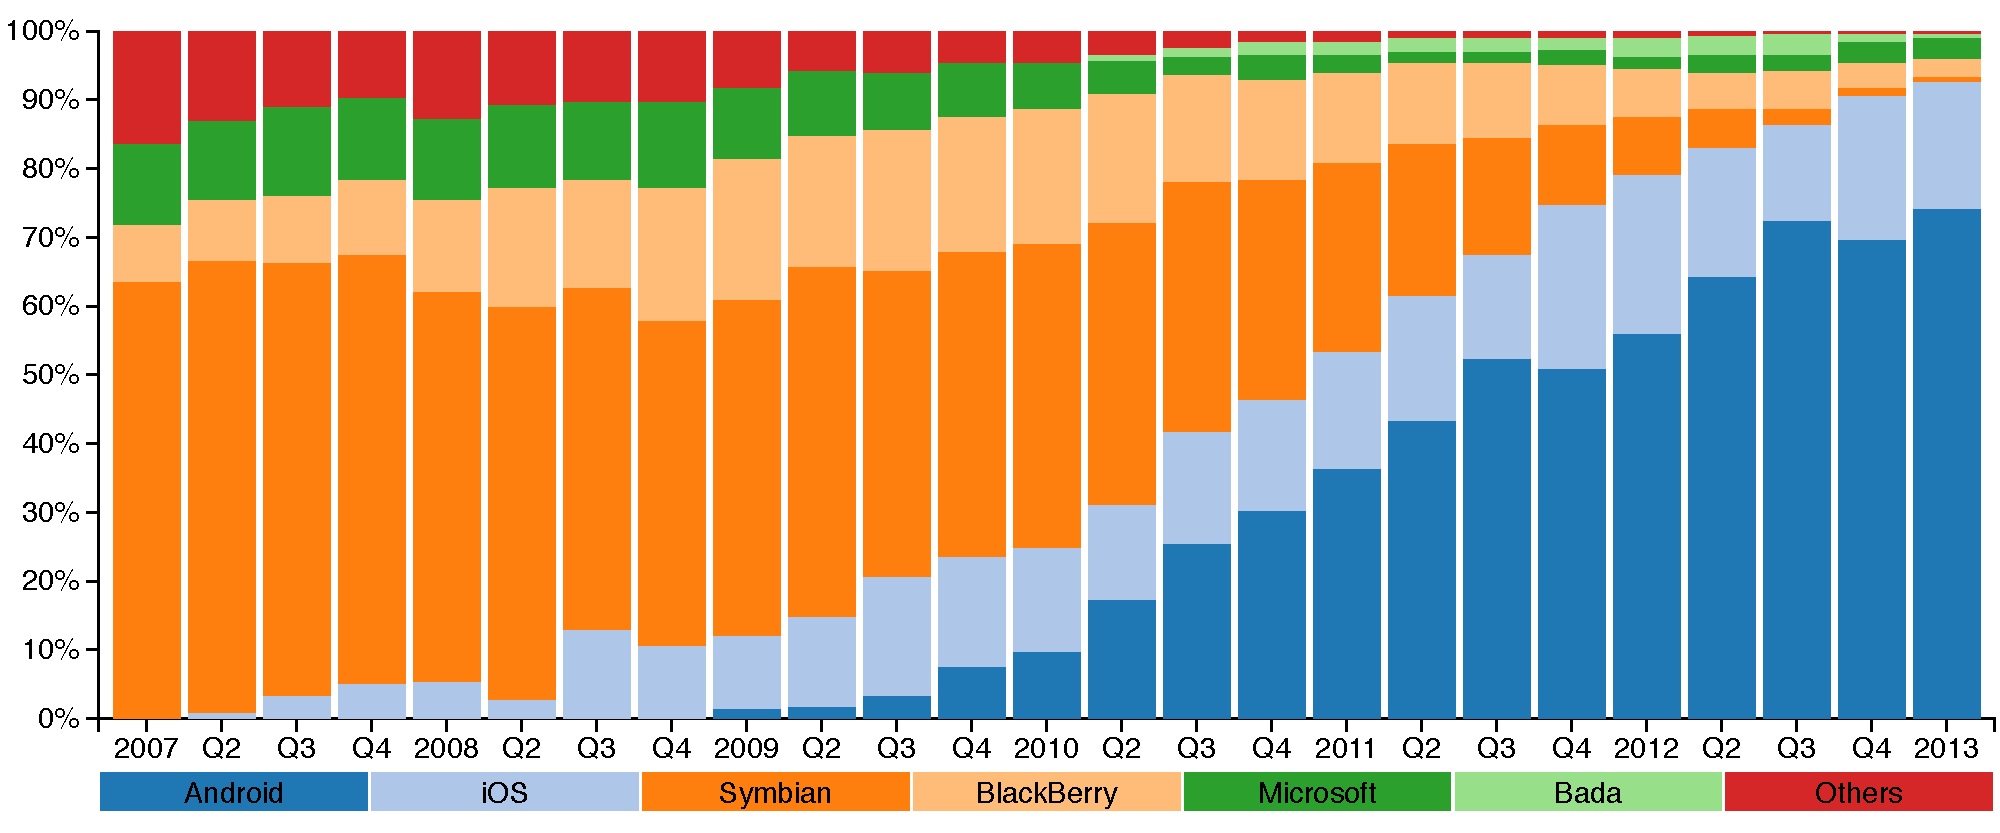
\includegraphics[width=\textwidth]{../resources/figs/smartphone_share.pdf}
    \caption{Evolution of worldwide smartphone market share by operating system.\newline Source: Gartner \citeGartner}
    \label{fig:smartphone-share}
\end{figure}

However, there is no single major platform. In addition, the IDC\footnote{International Data Corporation is another American research, analysis and advisory firm, specializing in information technology, telecommunications and consumer technology, \url{http://www.idc.com}.} predicts that Windows Phone will gain a significant market share by 2016 and that 90\% of the worldwide smartphone market will then be covered by Android, iOS and Windows Phone \cite{IDC:phone}. Hence, it is reasonable to assume that there will always be more than one major platform.

The second type of mobile devices are tablet computers or tablets. In their current form, tablets are somewhat similar to smartphones but they have larger touchscreens (customarily starting at 7 inches in diagonal) and do not offer basic telephony. However, some of them do have a cellular radio that can be used for data transmission. Because of their hardware similarities, their software is also similar: the dominant smartphone operating systems are also used in tablets.

As with smartphones, tablets gained a lot of popularity since the launch of the iPad and Android tablets. According to other studies by both Gartner \citep{Gartner:11tab,Gartner:12tab} and the IDC \citep{IDC:tablet}, tablets will continue to gain popularity and sales will be mainly driven by iPads and Android tablets (see \fref{fig:tablet}). Even though these studies disagree on which operating system will be used in most devices, they both predict there will be three major platforms: iOS, Android and Windows. 

\begin{figure}[h]
    \centering
    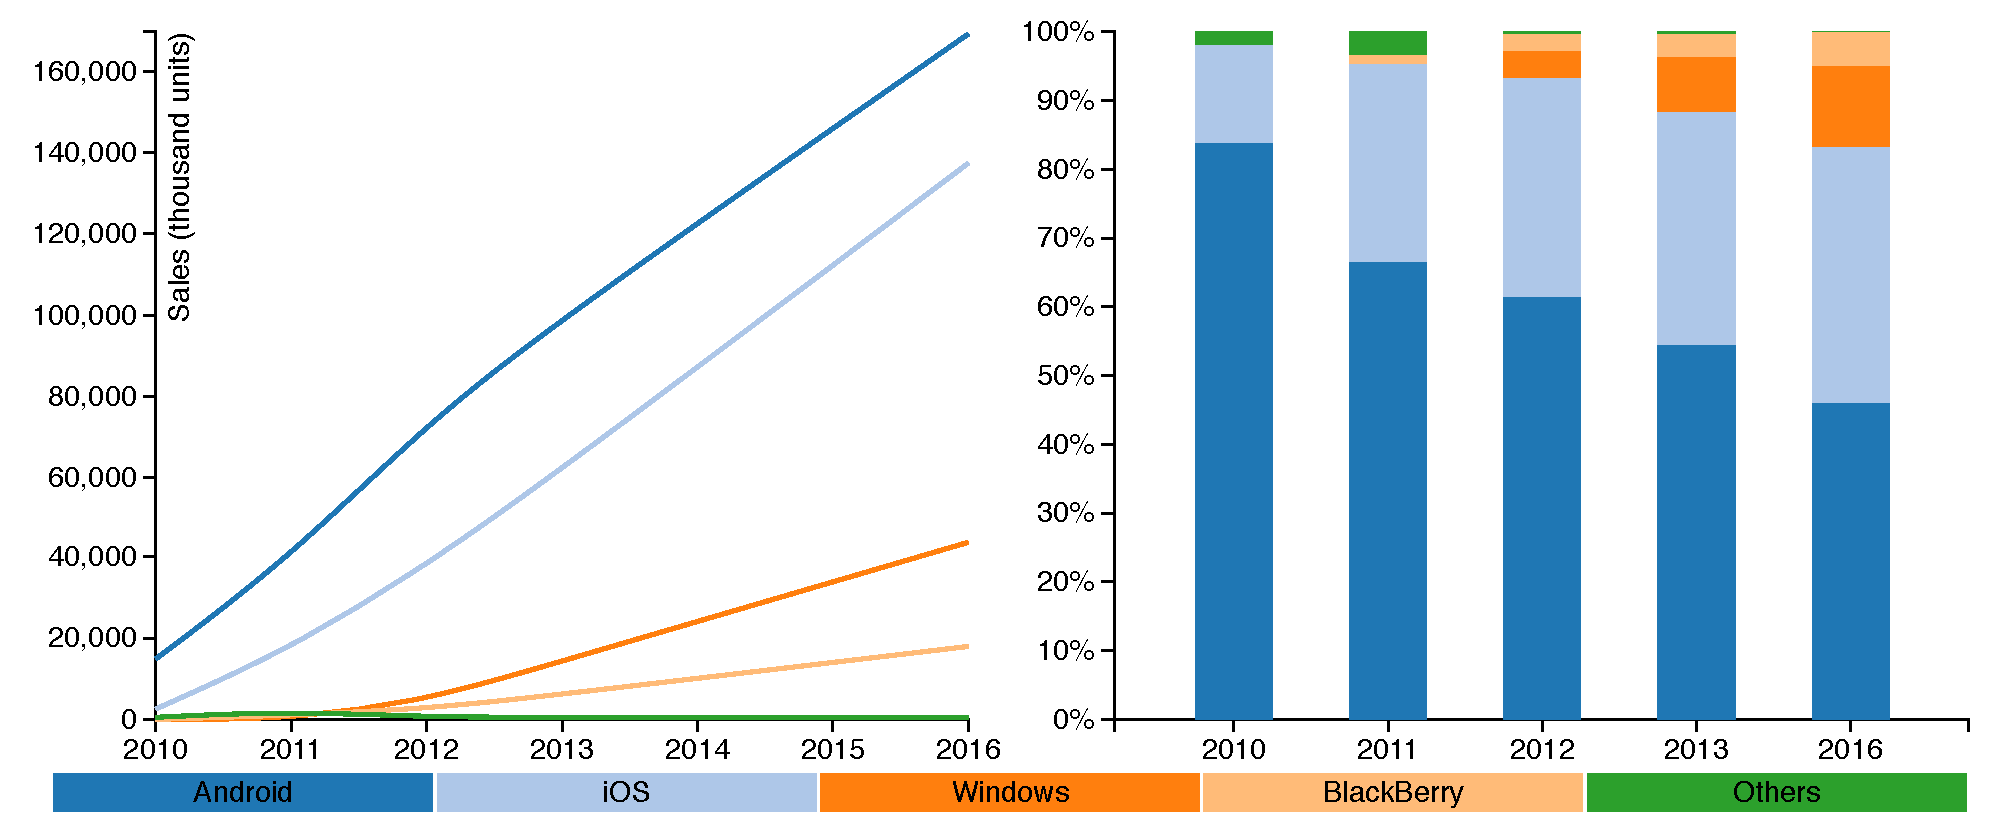
\includegraphics[width=\textwidth]{../resources/figs/tablet_sales.pdf}
    \caption{Prediction of worldwide tablet sales and market share.\newline Source: Gartner \citeGartnerTab}
    \label{fig:tablet}
\end{figure}

\section{The problem of fragmentation}

Fragmentation can be defined as the fact that all devices are different; there is no uniform device. This is called device fragmentation. In fact, all mobile devices can be divided into multiple, overlapping categories like operating system or platform (called platform fragmentation), operating system version or runtime (called runtime fragmentation), screen size and screen resolution (called screen fragmentation) and many more. Hence, fragmentation is a multi-dimensional problem. 

Fragmentation is generally beneficial for consumers, carriers and manufacturers. The more different devices there are, the more likely a consumer will find a device that fits his needs. For developers on the other hand, fragmentation is usually disadvantageous. It forces them to test their applications on multiple devices to guarantee the desired user experience. This is expensive and time-consuming. 

The nature of a platform strongly influences the fragmentation issues within said platform. For instance, Apple can manage fragmentation issues pretty well because iOS is a closed platform and the only devices running iOS, called iDevices, are designed by Apple itself. In fact, these devices show many similarities. Android on the other hand is an open system. Android is being developed privately at Google, but the source code of every release is publicly available under the Apache 2.0 License, which means that everybody is allowed to customize it. The ability for manufacturers to alter the operating system has largely contributed to the success of Android. 

Mobile device manufacturers are eager to modify the Android operating system to differentiate their product from their competitors. As such, they create their own Android flavour, i.e. a distribution of Android with a custom user interface (like HTC Sense, Samsung TouchWiz, etc.), custom software, additional market places, etc. However, reapplying these modifications for every new release of Android is cumbersome and costly which is why device manufacturers do not often provide updates for their devices. This has led to the notorious Android runtime fragmentation, which is depicted in \fref{fig:android_runtimes}. The adoption rate for new versions is low and is caused by the nature of Android. Developers have to support multiple versions, which is tedious. 

\begin{figure}[h]
    \centering
    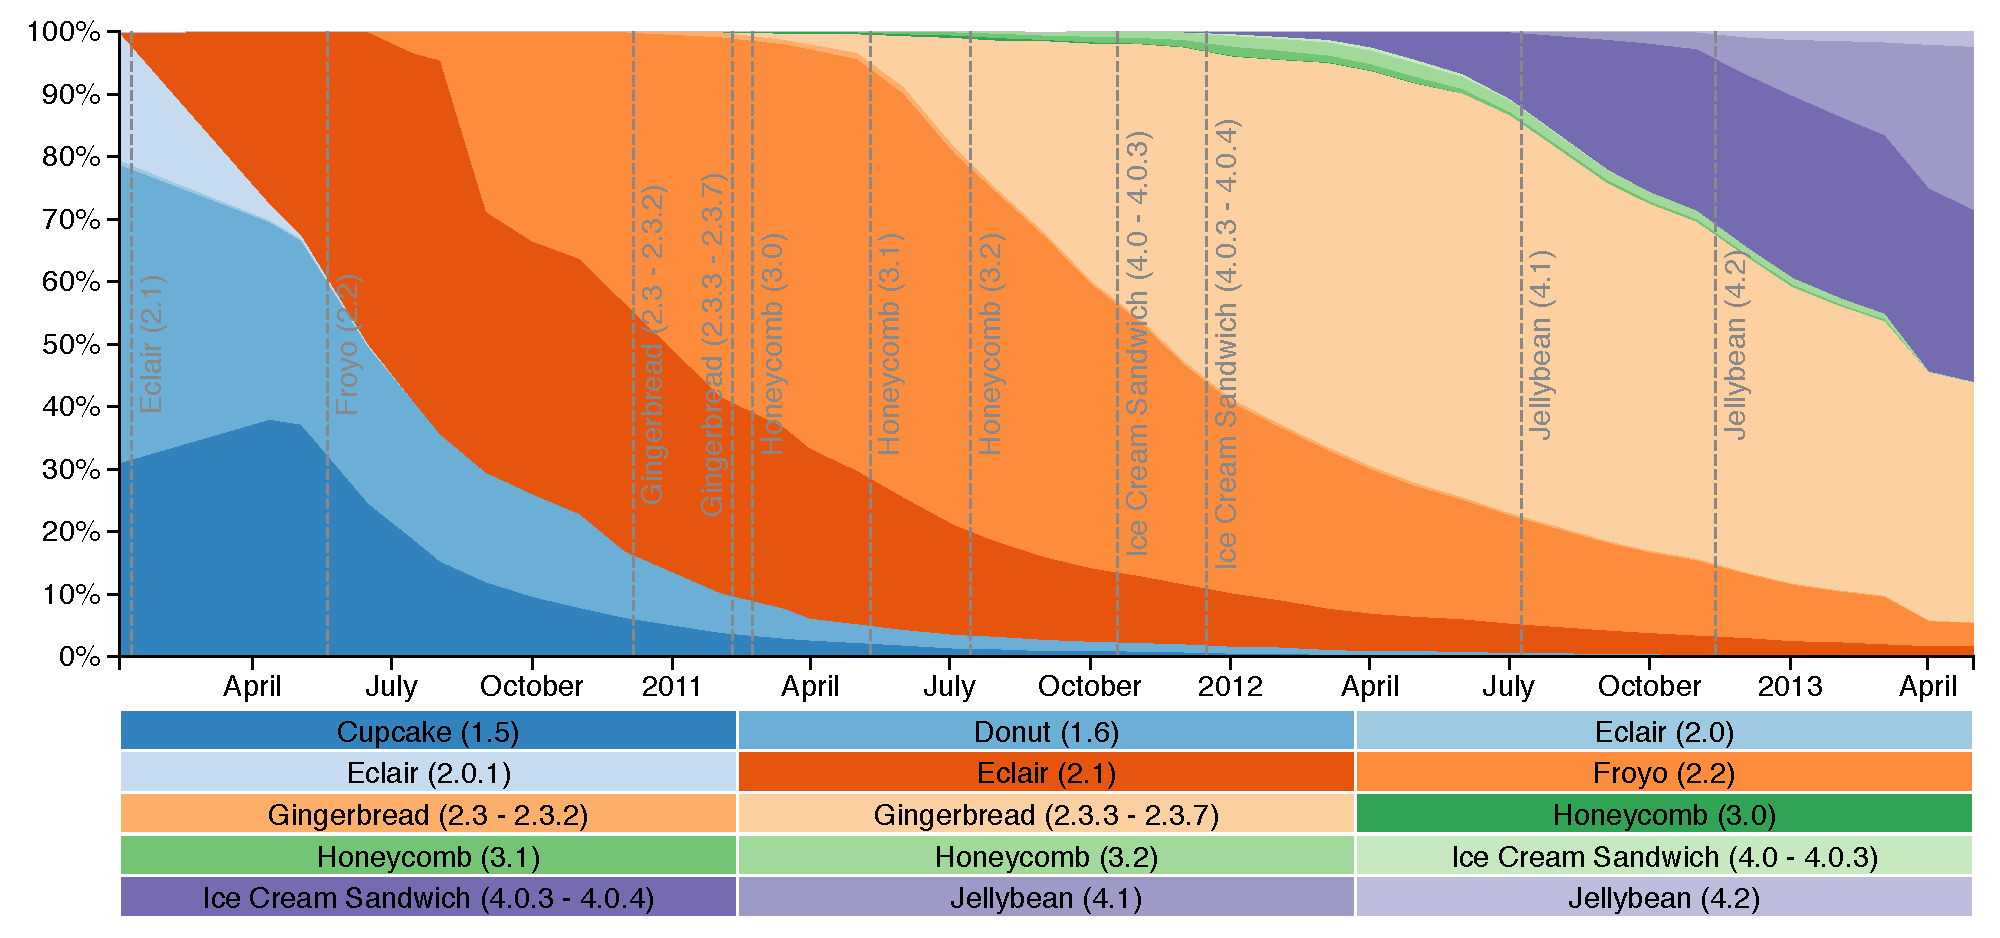
\includegraphics[width=\textwidth]{../resources/figs/android_runtimes.pdf}
    \caption{Historical Android runtime fragmentation. The data for this graph was aggregated from \cite{Android:Versions} using the Internet Archive (\url{http://archive.org}).}
    \label{fig:android_runtimes}
\end{figure}

Unlike Google, Apple does not publicize runtime statistics but developers \cite{Smith:2013} and online advertisers \cite{Chitika:2013} can confirm fast adoption rates for iOS. On iOS, developers can make use of new functionality much faster. However, as Apple starts to drop support for some of its devices that are still in use (like for instance the original iPad and the iPod third generation), it introduces runtime fragmentation. Because of this, iOS developers will have to support the latest two versions of iOS.

Android and iOS are used in both smartphones and tablets. There are only few different iDevices  but in contrast, there is an enormous number of Android devices. The Google Play Store\footnote{Google Play is the official marketplace for Android applications.} supports 2935 different device configurations, distributed across 63 manufacturers. All these devices come  with varying screen sizes and resolutions which implies that applications also have to deal with this. On Android, this is solved by a flexible layout system. On iOS, this is solved by centering the user interface in the middle of the screen. For instance, applications that are not optimized for the 4-inch display of the iPhone 5 (or iPod Touch, 5th generation) will have black bars on the top and the bottom. High-density displays\footnote{A high-density display has about twice the pixel density of a regular display.}, like the Retina display, do not really introduce a new screen resolution because every logical pixel is represented by four physical pixels and this conversion is mostly handled by the operating system.

There are still a lot more dimensions to the fragmentation problem like computing power, available sensors, available networking, etc. but these differences can be categorized under device fragmentation. In conclusion, fragmentation among Android devices is rather high compared to iDevices.

\section{Cross-platform tools to the rescue}

In the current economy, information is a company's most valuable asset and the rate at which information exchange takes place increases every day. Mobile Internet-enabled devices are a valuable resource for this purpose and, as a consequence, many companies want mobile applications for their businesses. However, in an ever-changing and unpredictable industry like the mobile industry, it is unwise to target a single platform. This could eventually lead to vendor lock-in, i.e. all operations (or a significant part thereof) are built on equipment or software of a single vendor which puts that vendor in a bargaining position. Companies will try to avoid these situations at all costs and they will do so by asking for cross-platform solutions. 

Making a solution work across platforms typically requires that the software has to be implemented multiple times: one time for each platform. This is costly and time-consuming. Cross-Platform Tools (CPTs) can help to solve this problem because they allow to support multiple platforms from a single codebase. Hence, they lower entry barriers (access to new platforms) and exit barriers (lock-in) \cite{VMCPT:2012}. 

Cross-Platform Tools try to solve three major problems \cite{VMCPT:2012}: 

\begin{enumerate}
    \item \textbf{Fragmentation} Fragmentation issues, as described above, are a struggle for every developer. They are forced to test their applications on a large number of devices in order to be able to guarantee the desired user experience. A CPT can help to identify platform quirks and provide workarounds. 
    \item \textbf{Access to new platforms} Targeting a new platform is generally hard. Developers have to learn yet another SDK and/or programming language in order to deliver applications for this platform. A CPT can make abstraction of platform differences which allows developers to reuse their current skills. This drastically reduces the effort that is needed to target a new platform. Bear in mind that a new platform does not necessarily have to be a smartphone or tablet operating system, it could also be the operating system of a television set, or a car console, etc.
    \item \textbf{Development inefficiency} Maintaining codebases for multiple platforms is a difficult and costly task. When a new feature is introduced, it has to be applied to all codebases. With the use of a CPT, all code is contained within a single codebase and no time is lost while synchronizing features and executing other maintenance tasks across codebases. This reduces cost while increasing productivity. 
\end{enumerate}

\section{Goals}

It is clear that there is a large demand for cross-platform solutions and that there are a lot of benefits associated with the use of cross-platform tools. Therefore, this thesis will try to identify a suitable cross-platform tool for mobile application development. This is a two-step process. First, a methodology will be defined for evaluating and selecting cross-platform tools. Second, this methodology will be used to evaluate two cross-platform tools (Apache Cordova and Motorola Rhodes) and the native SDK's in a business environment, provided by Capgemini\footnote{Capgemini is a multinational IT consulting company, \url{http://www.capgemini.com}.}. From this evaluation, the best-suited alternative will be selected. 
\chapter{Literature study}
\label{chap:literature}

This chapter presents an overview of literature that is related to this work. The first section will summarize the mobile application architectures that are currently used to create cross-platform solutions. In the second section, a generic software evaluation and selection methodology will be explored. In the third and last section, a number of techniques for multi-criteria decision making are studied, together with their strengths and weaknesses.

\section{Mobile application architectures}

Building cross-platform solutions starts at the architectural level. This section will discuss the architectures that are currently used with mobile applications or apps for short \cite{Friese}. Mobile architectures comprise of three key elements: 

\begin{itemize}
    \item The \emph{mobile device} is the piece of hardware that runs the actual application. This is the place where the architectures will differ the most.
    \item The \emph{backend} is a service, provided by one or more servers that store all the application data. This could be a web service, ERP software like SAP, a CRM system like Salesforce, etc. or it could be a combination of such services.
    \item The \emph{mobile hub} or\emph{mobile orchestrator} is a server that acts as a mediator between the mobile device and the backend. It is put in place for multiple reasons: it exposes a uniform interface to the mobile device (and hides external API changes), prevents distributed denial-of-service (DDoS) attacks from the large number of mobile devices connecting to the backend, can cache information to reduce the load on the backend, can inject services like advertising into the application, etc.
\end{itemize}

The architecture of the native application is discussed first and is used as a reference architecture. For each of these architecture, a number of aspects will be highlighted: performance, look \& feel, platform access, programming languages, development cost and distribution.

\subsection{Native application}

A native application is an application that is specifically designed to run on a particular platform. It is the default approach to develop applications for mobile devices and is therefore considered the reference architecture in this section. It is illustrated in \fref{fig:native}. 

\begin{figure}[h]
    \begin{center}
        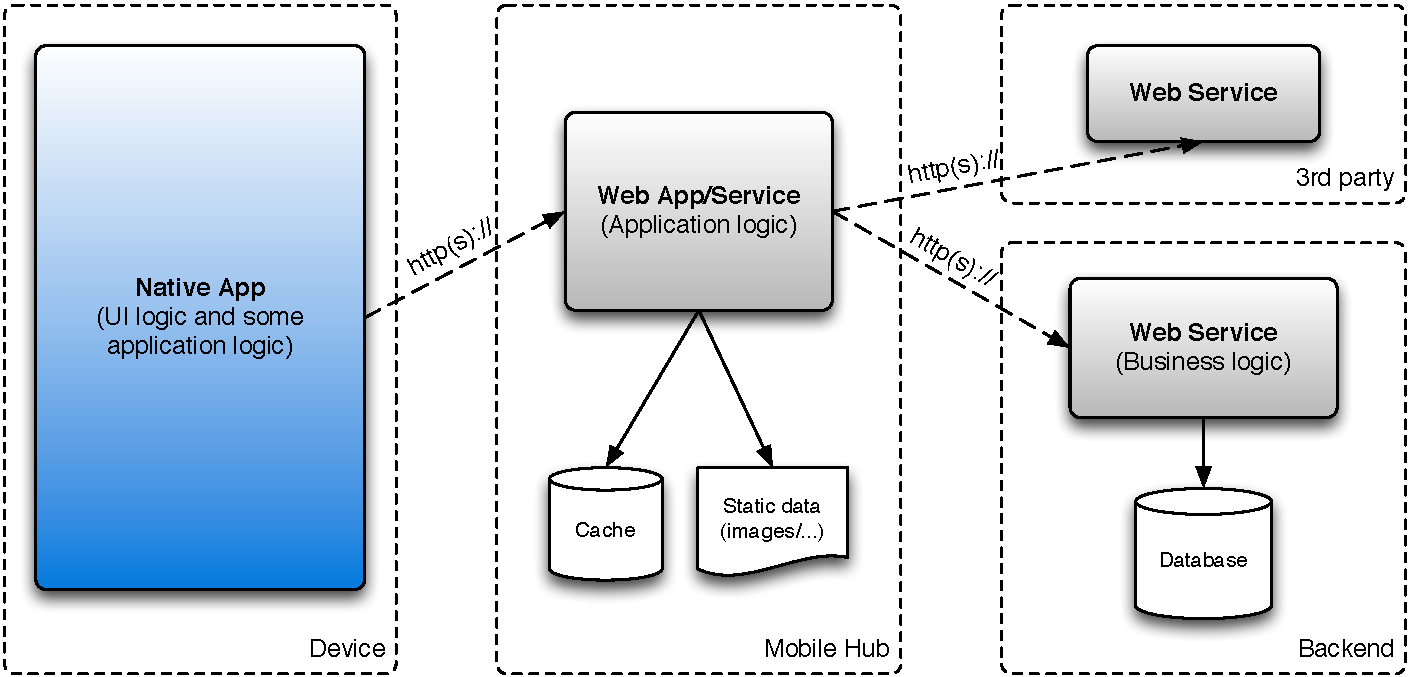
\includegraphics[width=\textwidth]{figs/native.pdf}
        \caption{Architecture of a native application. Based on \cite{Friese}}
        \label{fig:native}
    \end{center}
\end{figure}

Native applications are developed with the supplied software development kit (SDK). That SDK uses a particular programming language that developers will have to learn together with the features of the SDK. In return they will get full access to the platform and its features. As a result, the best performance can be achieved with this kind of application.

The SDK also provides a large number of user interface elements that developers can use to create a rich user interface that is consistent with the look \& feel of the platform. This is called native look \& feel. Native apps are typically distributed through an online marketplace like the App Store for iOS applications or Google Play for Android applications. 

The development cost of native applications is high because developers need to be familiar with multiple SDKs and the application has to be developed separately for every platform that has to be supported.

\subsection{Mobile web application}

Mobile web applications are websites that are optimized for mobile browsers. Since every platform comes with a browser, this is the easiest way to get an application running on all platforms. An overview of this architecture is depicted in \fref{fig:web}. Mobile web applications are built with HTML (content), JavaScript (behaviour) and CSS (styling, are viewed in the browser and are distributed on the Internet with a URL but they cannot be installed on the device. A workarounds using Web Clips \cite{Safari:webclips} is available on iOS and on Android, bookmarks can be placed on the home screen. 

\begin{figure}[h]
    \begin{center}
        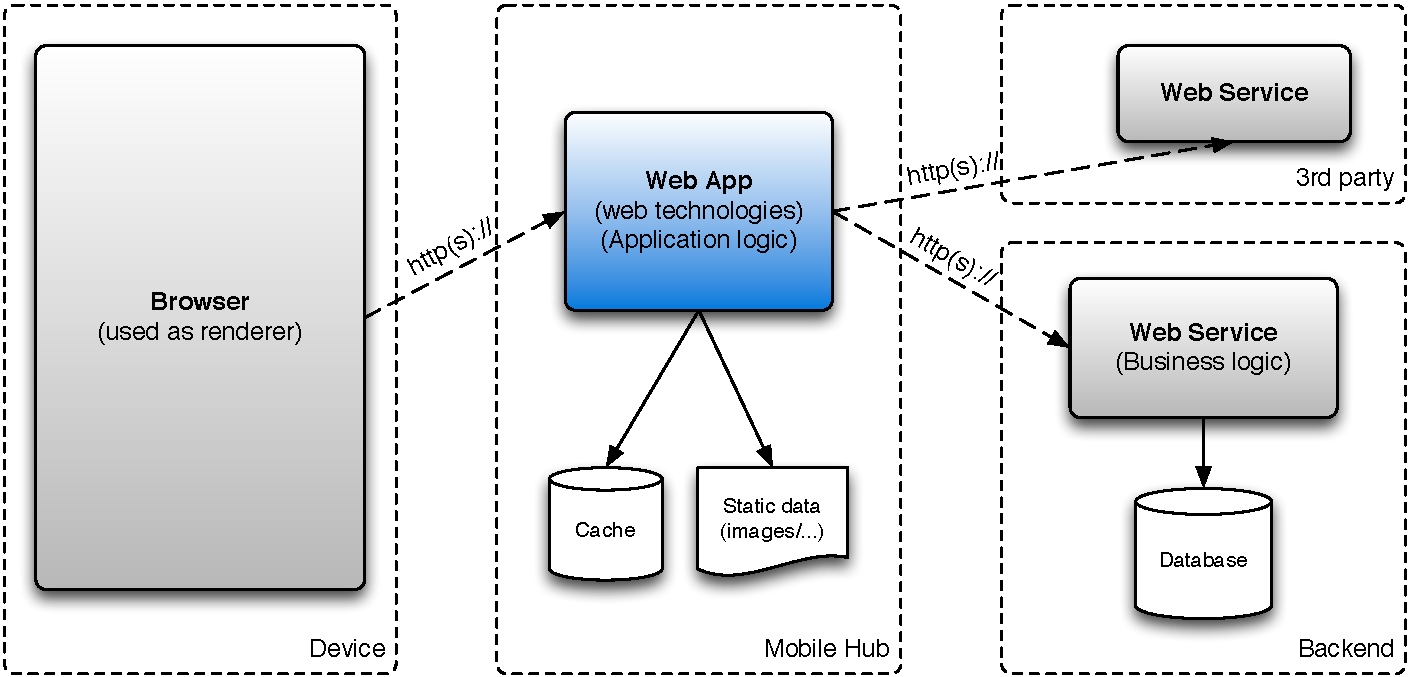
\includegraphics[width=\textwidth]{figs/web.pdf}
        \caption{Architecture of a mobile web application. Based on \cite{Friese}}
        \label{fig:web}
    \end{center}
\end{figure}

Mobile web applications are not nearly as powerful as native applications because the web is currently not a first-class platform. Many mobile web browsers lack support for particular HTML5 features. These defects are listed on websites like ``Can I use...''\footnote{\url{http://caniuse.com}} and ``Mobile HTML5''\footnote{\url{http://mobilehtml5.org}}. Developers should constantly check whether a certain feature is available. In some cases, the missing feature can be \emph{polyfilled}. This term polyfill is inspired by the famous wall filler ``Polyfilla'' and is used for additional pieces of code that provide the missing HTML5 functionality. However, no polyfill can provide access to the underpinning hardware. Most mobile web applications also require an internet connection because the application is not cached in the browser. 

Mobile web applications cannot make use of the native user interface elements. Because of this limitation, it is hard to provide a native look \& feel. There are a number of project that try to mimic the native user interface elements with HTML templates and custom styles. However, the styling is quite complex and additional behaviour is added to animate these elements, which is disadvantageous for the performance. On the other hand, some people believe that the web is a platform of its own because it satisfies the ``one size that fits all'' philosophy. Therefore, it is entitled to its own look \& feel \cite{Mahemoff:2011}.

The development cost of mobile web applications is low because it does not require additional skills (web development is often already in the skill portfolio) and the application has to be developed only once and can serve all platforms. 

\subsection{Hybrid application}

A Hybrid application is the combination of a native application and a mobile web application. The actual application is a mobile web application that is embedded in a native application and made visible through a WebView\footnote{A WebView is a native user interface element that displays web content inside applications.}. The native shell offers a JavaScript bridge to the web application, allowing the web application to access to the system. Because hybrid applications and wrapped in a native shell, they can be distributed through (official) marketplaces. The architecture is visualized in \fref{fig:hybrid}.

\begin{figure}[h]
    \begin{center}
        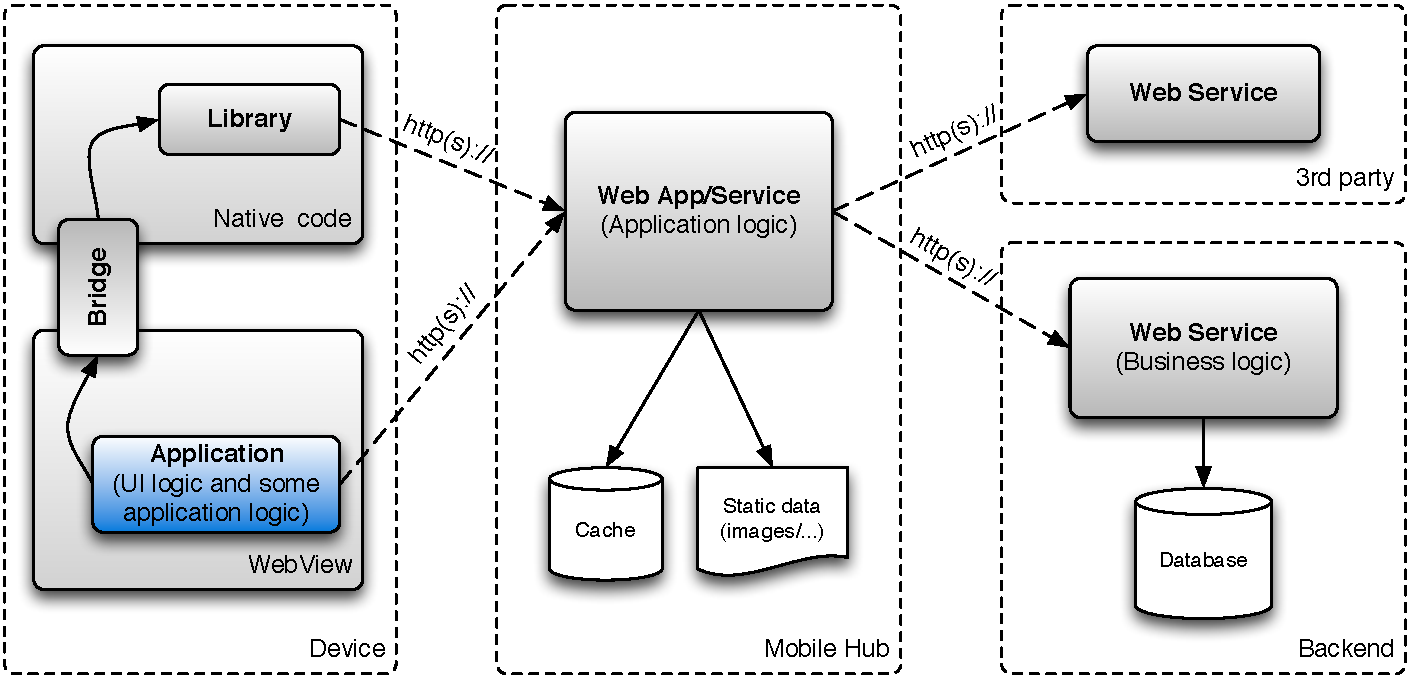
\includegraphics[width=\textwidth]{figs/hybrid.pdf}
        \caption{Architecture of a hybrid application. Based on \cite{Friese}}
        \label{fig:hybrid}
    \end{center}
\end{figure}

Because of the nature of the application, the performance is be similar to web applications. Unlike mobile web applications, hybrid applications are more flexible because they allow better integration with the device through the JavaScript bridge. This way, missing features can be implemented natively and accessed through said bridge. Another consequence of its nature is that hybrid applications do not use the native user interface elements and cannot provide the native look \& feel. 

The development cost of hybrid applications is similar to that of mobile web applications because wrapping web applications does not require any knowledge of the native SDK's. 

\subsection{Interpreted application}

Interpreted or runtime applications try to solve the platform differences by introducing an intermediary programming language. Instructions from that language are translated to native instructions at runtime. Interpreted applications are similar to Java applications on the desktop. From the outside, interpreted applications look just like native applications and can be distributed through online marketplaces. An interpreter or runtime is built right into the application, which increases the installation size of the application. This could be disadvantageous on low-end smartphones with limited storage capabilities. The architecture of an interpreted application is demonstrated in \fref{fig:interpreted}.

\begin{figure}[h]
    \begin{center}
        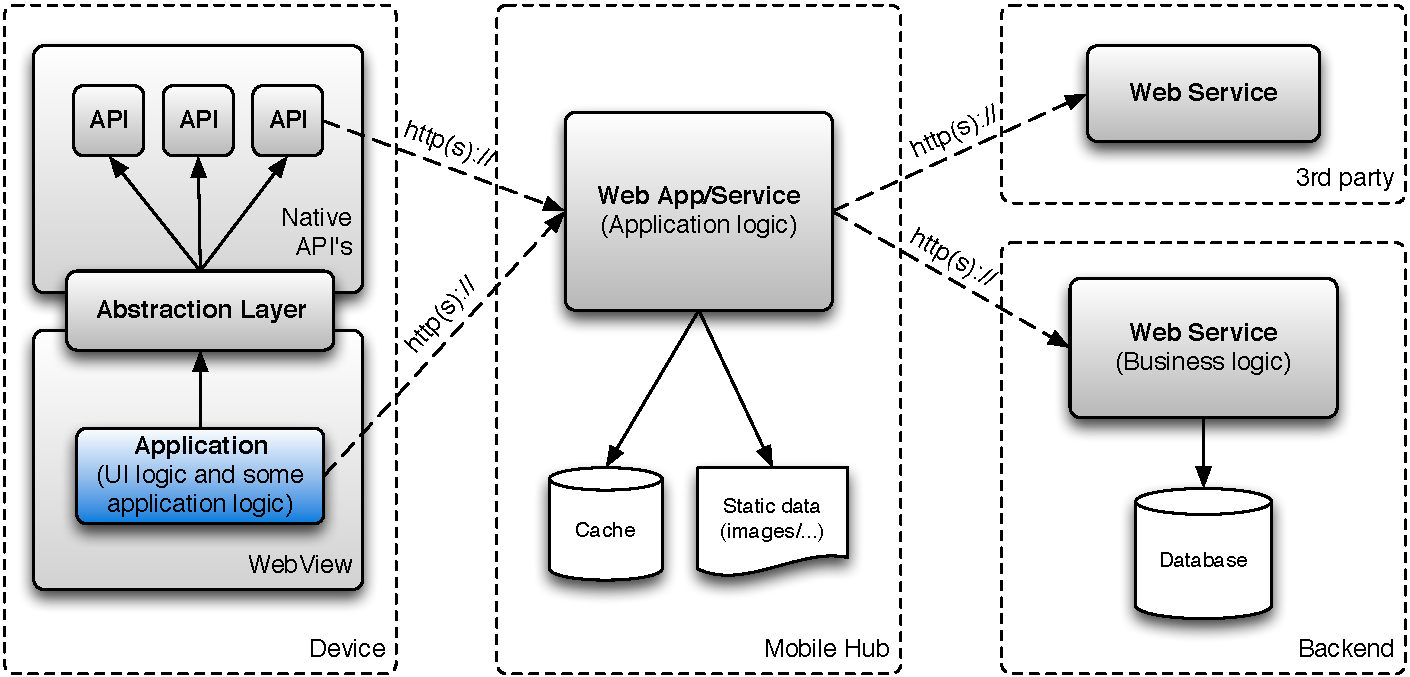
\includegraphics[width=\textwidth]{figs/interpreted.pdf}
        \caption{Architecture of an interpreted or runtime application. Based on \cite{Friese}}
        \label{fig:interpreted}
    \end{center}
\end{figure}

The performance of an interpreted application strongly depends on the interpreter itself and the interpreted programming language. In general, the performance is better than the performance of web applications but it is not as good as the performance of native applications. Because of the nature of interpreted applications, the native user interface elements can be used to provide a native look \& feel.

The development cost of interpreted applications is a higher than the cost of mobile web applications but lower than the cost of native applications. Developers need to be familiar with the SDK of the cross-platform tool but the application has to be developed only once and can be run on all supported platforms.

\subsection{Cross-compiled application}

In contrast to interpreted applications, instructions of cross-compiled are translated at compile time. The resulting application is not noticeably different from a native application because no runtime has to be included. This architecture is presented in \fref{fig:crosscompiled}. 

\begin{figure}[h]
    \begin{center}
        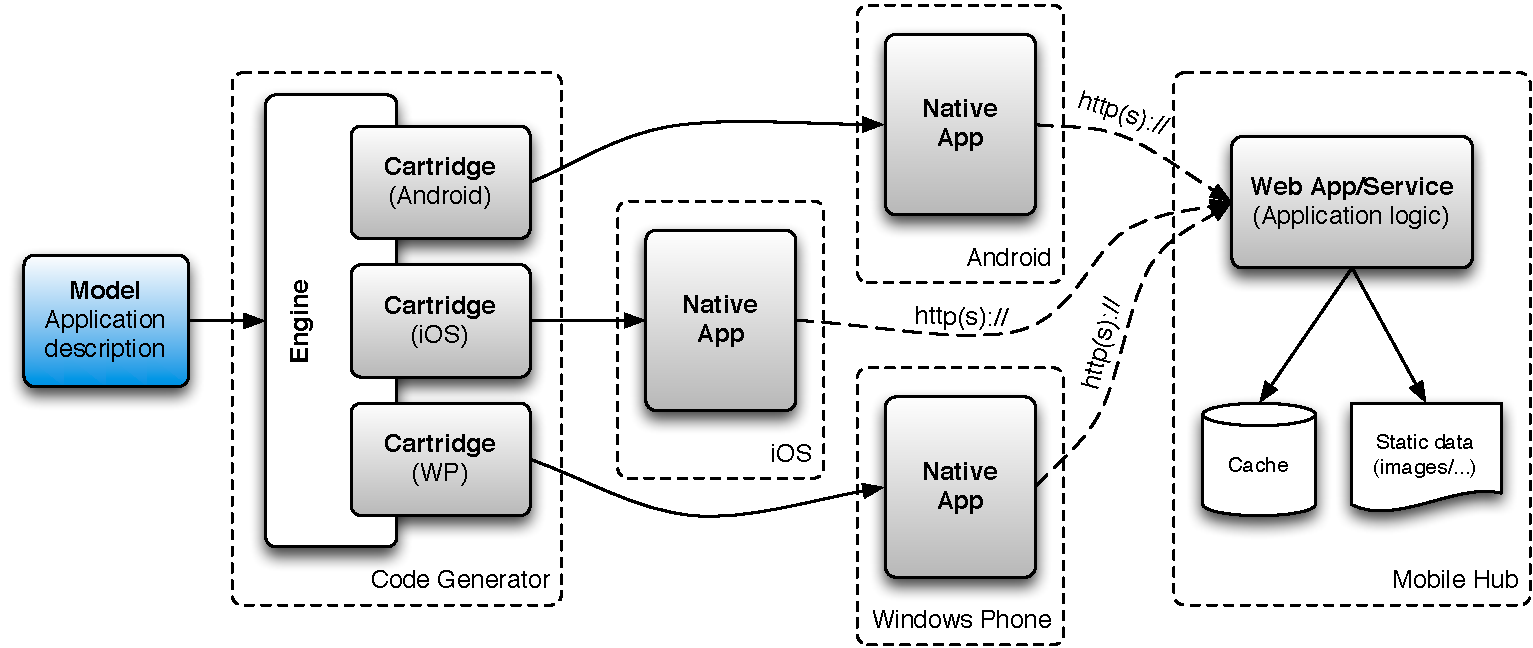
\includegraphics[width=\textwidth]{figs/crosscompiled.pdf}
        \caption{Architecture of a cross-compiled application. Based on \cite{Friese}}
        \label{fig:crosscompiled}
    \end{center}
\end{figure} 

Because the application only exists of machine code, the performance of cross-compiled applications is nearly identical to the performance of native applications. Cross-compiled applications can make use of the native user interface elements and consequently provide the native look \&feel. However, this sometimes requires custom bindings for each platform, increasing the amount of code that has to be written. 

The development costs of cross-compiled applications is similar to the costs of interpreted applications. Developers still need to be familiar with the SDK of the cross-platform tool but the application has to be developed only once and can be run on all supported platforms. Also, not all code can be reused in cross-compiled applications, which raises the development costs a little more.

\subsection*{Comparison of mobile architectures}

To conclude this section, the discussed architectures are compared side by side. The results are shown in \tref{tab:architectures}. Every architecture has both strengths and weaknesses. Therefore, the architecture must be chosen carefully, taking the client's wishes into account. 

\begin{table}[h]
    \begin{center}
        \begin{tabular}{lccccc}
            \hline
                            & Native      & Web         & Hybrid      & Interpreted & Cross-compiled\\
            \hline
            Performance     & high        & low         & low         & average     & high          \\
            Hardware access & \checkmark  & partial     & \checkmark  & \checkmark  & \checkmark    \\
            Look \& Feel    & native      & non-native  & non-native  & native      & native        \\
            Distribution    & store       & URL         & store       & store       & store         \\
            Cost            & high        & low         & low         & moderate    & moderate      \\
            \hline
        \end{tabular}
		\caption{
			Summary of cross platform mobile application development strategies.
		}
		\label{tab:architectures}
    \end{center}
\end{table}

\section{Software evaluation methodology}
\label{sec:sw-selection}

One of the goals of this thesis is to design a methodology for evaluating and selecting cross-platform tools. Based on their literature review \cite{Jadhav:2009}, \citet{Jadhav:2011} propose a generic software selection methodology. This methodology comprises of six steps:

\begin{enumerate}
    \item \textbf{Define selection criteria.} In the first stage, the selection criteria are defined. These are the functional and non-functional requirements that a software package has to meet.
    \item \textbf{Identify potential candidates.} During the second stage, a list of potential candidates is composed. During this search, any package that could be used to solve the targeted problem is considered a potential candidate. 
    \item \textbf{List selected alternatives.} In the third step, the selection criteria from the first stage are used to filter the list of potential candidates from the second stage: if a candidate does not satisfy the selection criteria, it is not considered for further evaluation.
    \item \textbf{Define evaluation criteria.} In the fourth stage, the evaluation criteria are defined. These are criteria that will be used to score a particular software package. These criteria should be arranged in a tree and every leaf node should be well-defined and measurable basic attribute.
    \item \textbf{Evaluate selected alternatives.} During the fifth phase, the software packages are evaluated. First, weights are assigned to the evaluation criteria from the fourth stage. Second, the software packages are rated with respect to the evaluation criteria. Third, an aggregated score is calculated for each software package.
    \item \textbf{Select the most suitable alternative.} In the final stage, all alternatives are ranked in order of decreasing aggregated score (which was calculated in the previous stage). The most suited software package will rank highest. However, selection is always human-dependable: additional cost-benefit analysis could be performed to identify the package with the best value, contract negotiations can influence the decision, etc. 
\end{enumerate}

In their first paper, \citet{Jadhav:2009} also suggest to include a validation stage to confirm that the selected package is indeed the most suited. 

\section{Multicriteria decision making (MCDM)}
\label{sec:mcdm}

The generic software selection methodology of \citet{Jadhav:2011} does not impose a particular technique for evaluating software packages. However, the last three stages of this methodology can be recognized as a multi-criteria decision making (MCDM) problem, for which a number of techniques are available. Multi-criteria decision making refers to making decisions in the presence of multiple --- often conflicting --- criteria. 

There are two types of MCDM problems: in multi-attribute decision making (MADM) problems, the decision maker tries to \emph{identify} the ``best'' alternative from a \emph{finite} set of alternatives with respect to multiple criteria or \emph{attributes}. In multi-objective decision making (MODM) problems, the decision maker tries to \emph{design} the ``best'' alternative from an \emph{infinite} set of possibilities with respect to multiple \emph{objectives} \cite{Kahraman:2008}. The software selection process clearly belongs to the category of MADM problems because the goal is to find the best alternative within a finite set of alternatives \cite{Jadhav:2009, Jadhav:2011}. 

There are numerous approaches to solve MADM problems. In the next subsections, a collection of approaches that are successfully applied in literature will be discussed. Every subsection will present a (high-level) description of the method and its strengths and weaknesses. Subsequently, every method is applied to a simple, running example.

The running example is as follows. Ethan has just graduated and has received three job offers. Every job is evaluated with respect to four criteria: the starting salary, distance to work (in km), degree of interest and career opportunities. Job 1 is an interesting position at a local start-up but it pays less. A large multinational offers job 2, which has a high reward and great career opportunities but is also further away from home. Job 3 is far away from home but combines great career opportunities with a good salary and interesting work. Note that the first two criteria are quantitative criteria, i.e. they can easily be mapped on a number. The last two criteria are qualitative criteria, i.e. they give a description but there is no straightforward mapping on a number. 

\subsection{Scoring models}

The first approach to solving MCDM problems is a collection of methods that have one thing in common: every alternative is assigned an arbitrary score with respect to one criterion and the scores for all criteria are aggregated into one final score. The final scores are then used to rank the alternatives.

Different methods are available to calculate the final score of a candidate \cite{Kahraman:2008}:

\begin{itemize}
    \item The ``dominance'' method can be used when one alternative  clearly outperforms the other alternatives with respect to at least one criterion and performs equally well with respect to the other criteria. 
    \item The ``maximin'' method calculates the total score of an alternative as the lowest score of all criteria scores of this alternative.
    \item The ``maximax'' method calculates the final score of an alternative as the highest score of all criteria scores of this alternative.
    \item With the ``conjunctive'' method, an alternative should exceed certain thresholds for \emph{all} criteria.
    \item With the ``disjunctive'' method, an alternative should exceed certain thresholds for \emph{at least one} criterion. 
    \item The ``additive weighting'' method calculates the total score of an alternative as the weighted \emph{sum} of the criteria scores and criteria weights.
    \item The ``weighted product'' method calculates the total score of an alternative as the weighted \emph{product} of the criteria scores and criteria weights.
\end{itemize}

The strength of these methods is that they are the easy to use. The weaknesses are that it (1) is hard to assign scores to qualitative criteria and definitely when there are many alternatives because humans can only deal with 7, plus or minus 2 pieces of information simultaneously and (2) different scales get mixed up \cite{Jadhav:2009, Miller:1956}. These weaknesses will become clear in the example.

\paragraph{Example}

Assume that Ethan has assigned weights to the four criteria in an arbitrary fashion and that he has also assigned scores to every alternative. Because this method requires a numerical value for each criterion, Ethan has created a value scale for ``interest'' and ``opportunities'': 0 represents satisfiable, 1 represents good and 2 represents excellent. Also, the distance property has been inverted such that a shorter distance is rewarded with a higher score. He has naively used the additive weighting method to aggregate the scores. The weights, scores, and resulting total scores are listed in \tref{tab:sm1}.

\begin{table}[h]
    \begin{center}
        \begin{tabular}{lrrrrr}
            \hline
            Alternative & Salary & Distance (km) & Interest & Opportunities & Total Score \\
            \hline
            Job 1       & 2000   & 1/5           & 2        & 0             & 400.62       \\
            Job 2       & 2800   & 1/30          & 0        & 2             & 560.80       \\
            Job 3       & 2600   & 1/60          & 1        & 1             & 520.70      \\
            \hline
            Weight      & 20\%   & 10\%          & 30\%     & 40\%          &             \\
            \hline
        \end{tabular}
        \caption{Naive demonstration of the additive weighting method.}
        \label{tab:sm1}
    \end{center}
\end{table}

From this first and naive attempt, Ethan would be inclined to choose the second job offer over the third one, and the third offer over the first one. However, there are a number of issues with this approach. The scores have different orders of magnitude, which affects the scaling. This can be solved by normalizing the scores, i.e. dividing each score by the sum of scores for a particular criterion. The new, normalized scores are listed in \tref{tab:sm2}.

\begin{table}[h]
    \begin{center}
        \begin{tabular}{lrrrrr}
            \hline
            Alternative & Salary & Distance (km) & Interest & Opportunities & Total Score \\
            \hline
            Job 1       & 0.27   & 0.80          & 0.67     & 0             & 0.33        \\
            Job 2       & 0.38   & 0.13          & 0        & 0.67          & 0.36        \\
            Job 3       & 0.35   & 0.07          & 0.33     & 0.33          & 0.31        \\
            \hline
            Weight      & 20\%   & 10\%          & 30\%     & 40\%          &             \\
            \hline
        \end{tabular}
        \caption{Improved version of the additive weighting method.}
        \label{tab:sm1}
    \end{center}
\end{table}

In the second attempt, the ranking of the alternatives has changed. This is caused by normalizing the scores before weighting. One problem remains unsolved though: the value scale for interest and opportunity criteria does not capture the distance between two successive values. The used scale is an ordinal scale, i.e. the elements of the scale have a well-defined order but the distance between elements is undefined. Scoring models are not suited to convert qualitative criteria into numbers.

\subsection{Analytic Hierarchy Process (AHP)}
\label{sec:ahp}

The second method is the Analytic Hierarchy Process (AHP) \cite{Saaty:1980}. This method, developed by Thomas L. Saaty, is widely used in multi-attribute decision making. The method can be used with both qualitative and quantitative criteria and calculates priorities (or weights) from pairwise comparison matrices by using the eigenvalue problem. 

The analytic hierarchy process consists of two stages. During the first stage, the factors that are important for the decision are organized into ``a hierarchic structure descending from an overall goal to criteria, subcriteria and alternatives in successive levels'' \cite{Saaty:1990}. Organizing the factors in such a structure helps the decision maker in getting an overview of the potentially complex relationships and also helps to assess the relative importance of the issues in each level. Structuring information in a tree is also backed by experiments of psychologist George Miller. He found that people can only deal with a few facts simultaneously; more precisely seven, plus or minus two \cite{Miller:1956}. 

During the second stage, both criteria and alternatives are compared in pairs. Every pairwise comparison results in a number that expresses the relation between two criteria or alternatives. \citet{Saaty:1990} proposes a fundamental scale (listed in \tref{tab:ahp-scale}) for expressing these relations. The results of the pairwise comparisons are combined in matrices and the analytic hierarchy process then establishes a ranking of the alternatives by calculating the principal right eigenvector of these comparison matrices. The next paragraphs will present an intuitive justification of the method.

\begin{table}
    \begin{center}
        \begin{tabular}{p{2.5cm}p{4cm}p{6cm}}
            \hline
            Intensity of importance on an absolute scale & Definition & Explanation \\
            \hline
            1 & Equal importance & Two activities contribute equally to the objective \\
            3 & Weak importance of one over another & Experience and judgement slightly favour one activity over another \\
            5 & Essential or strong importance & Experience and judgement strongly favour one activity over another \\
            7 & Very strong or demonstrated importance & An activity is favoured very strongly over another; its dominance is  demonstrated in practice \\
            9 & Absolute importance & The evidence favouring one activity over another is of the highest possible order of affirmation \\
            2, 4, 6, 8 & Intermediate values between adjacent scale values & When compromise is needed \\
            Reciprocals of above nonzero & \multicolumn{2}{p{10cm}}{If activity $i$ has one of the above nonzero numbers assigned with activity $j$, then $j$ has the reciprocal value when compared with $i$. This is a reasonable assumption.} \\
            Rationals & Ratios arising from the scale & If consistency were to be forced by obtaining $n$ numerical values to span the matrix \\
            \hline
        \end{tabular}
        \caption{The fundamental scale for pairwise comparison\cite{Saaty:1990}}
        \label{tab:ahp-scale}
    \end{center}
\end{table}

Consider $n$ alternatives $A_1, A_2, \ldots, A_n$ and a quantitative criterion $X$, i.e. $X$ can be expressed with an exact number. The value of a certain alternative $A_i$ with respect to criterion $X$ is given by $w_i$. For instance, $A_i$ could be $n$ stones and $X$ could be their weight, measured in grams. The ratios between any two alternatives (with respect to property $X$) can now be summarized in a matrix
\begin{gather*}
    A = %
    \begin{bmatrix}
        w_1/w_1 & w_1/w_2 & \ldots & w_1/w_n \\
        w_2/w_1 & w_2/w_2 & \ldots & w_2/w_n \\
        \vdots  & \vdots  &        & \vdots  \\
        w_n/w_1 & w_n/w_2 & \ldots & w_n/w_n    
    \end{bmatrix}.
\end{gather*}

Note that (1) $A$ is reciprocal, i.e. $a_{ij} = 1 / a_{ji}$ and (2) the elements on the diagonal are ones. This is easy to understand because there cannot be any difference between two identical objects.

If any row of $A$ were to be multiplied by a vector $\vec{w} = (w_1, w_2, \ldots, w_n)^T$, the multiplication would yield a row of identical entries $w_i, w_i, \ldots, w_i$. This is only true in the case of perfect information. In most multi-criteria decision making problems, information is incomplete, incorrect or it simply cannot be represented by numbers (because the criterion describes a qualitative property) and the exact ratios cannot be calculated. In that case, the ratios $a_{ij} = w_i/w_j$ can be estimated by an expert, who is allowed to make (small) errors in judgement. These estimates $a'_{ij}$ make up a new matrix $A'$. Then, the result of the aforementioned multiplication is a row of statistically scattered values around the actual value $w_i$. Therefore, it seems reasonable to represent $w_i$ by the average of these values:
\begin{gather*}
    w'_i = \frac{1}{n} \sum_{j=1}^{n} a'_{ij} w'_j \quad i = 1, 2, \ldots, n
\end{gather*}

This resulting system can be solved for $\vec{w'} = (w'_1, w'_2, \ldots, w'_n)^T$ if $n$ is allowed to change. The problem then reads:
\begin{gather*}
    w'_i = \frac{1}{\lambda_{max}} \sum_{j=1}^{n} a'_{ij} w'_j \quad i = 1, 2, \ldots, n
\end{gather*}
which is equivalent to the eigenvalue problem $A' \vec{w'} = \lambda_{max} \vec{w'}$. The eigenvector $\vec{w'}$, which is unique up to within a multiplicative constant, has to be normalized by dividing its entries by their sum to obtain a \emph{priority vector}, i.e. a vector of appropriate weights or scores for the considered alternatives. 

The eigenvalue problem has a number of interesting properties. Reconsider $A$. This is a positive, reciprocal matrix and it is also consistent, i.e. all entries satisfy the condition
\begin{gather*}
    a_{jk} = \frac{a_{ik}}{a_{ij}} = \frac{w_i}{w_k} \times \frac{w_j}{w_i} \quad i, j, k = 1, \ldots, n.
\end{gather*}
In other words, the alternatives form a chain which also represents their ranking. Because of this property, all rows of $A$ are linearly dependent and consequently, $A$ has rank one. This also implies that all eigenvalues are zero, except one. In every matrix, the sum of eigenvalues is equal to the sum of elements on the diagonal (also known as the trace of a matrix). Hence, $tr(A) = n$, the order of $A$.

In the presence of small inconsistencies (where $A$ is approximated by $A'$), $\vec{w'}$ is a good estimate of $\vec{w}$ as long as $A'$ is reciprocal because it can be shown that small perturbations of $a_{ij}$ do not lead to large perturbations of $\lambda_{max}$ and $\vec{w'}$ \cite{Saaty:1980}. However, the amount of inconsistency should be measurable in order to decide whether it is small or not. It turns out that the amount of inconsistency is proportional to the difference between the expected eigenvalue $n$ and the actual eigenvalue $\lambda_{max}$.

\citet{Saaty:1980} defines a number, called the \emph{consistency index}, $CI = (\lambda_{max} - n) / (n - 1)$, which measures the amount of inconsistency in a given judgement matrix. This consistency index is then compared to the average consistency index of a large number of random reciprocal matrices of the same order, called the \emph{random index} (RI). These random indices can be found in \tref{tab:ri}. If the \emph{consistency ratio} $CR = CI / RI$ is $0.1$ or less, the estimate $\vec{w'}$ is accepted. Otherwise, new judgements should be collected in order to improve consistency.

\begin{table}
    \begin{center}
        \begin{tabular}{l*{9}{|c}}
            n & 1 & 2 & 3 & 4 & 5 & 6 & 7 & 8 & 9\\
            \hline
            RI & 0 & 0 & 0.58 & 0.90 & 1.12 & 1.24 & 1.32 & 1.41 & 1.45
        \end{tabular}
        \caption{Random indices (RI) for reciprocal matrices of order 1 to 9}
        \label{tab:ri}
    \end{center}
\end{table}

The strengths of the AHP are that it (1) enables decision makers to structure a problem into a hierarchy, (2) provides a powerful approach for handling both quantitative and qualitative criteria and (3) can deal with inconsistencies. The weaknesses of AHP are that it (1) is a time-consuming method due to the large number of pairwise comparisons and (2) is susceptible to rank-reversal, i.e. the ranking may change when new alternatives are added \cite{Jadhav:2009}.

\paragraph{Example}

In this example, Ethan uses the AHP method to assist him in choosing a job offer. The goal, which is the root node of the hierarchy, is obviously to select a job offer. The four criteria (salary, distance to work, interest and career opportunities) are children of the root node and the alternatives are children of the criterion nodes. \fref{fig:ahp-hierarchy} illustrates the hierarchy.

\begin{figure}
    \begin{center}
        \begin{pspicture}(0, 0)(12, 4)
            \psnode(6, 4){G}{Goal}
            \psnode(2.4, 2){C1}{Salary}
            \psnode(4.8, 2){C2}{Distance}
            \psnode(7.2, 2){C3}{Interest}
            \psnode(9.6, 2){C4}{Opportunities}
            \psnode(3, 0){O1}{Offer 1}
            \psnode(6, 0){O2}{Offer 2}
            \psnode(9, 0){O3}{Offer 3}
            
            \ncline[nodesep=3pt]{G}{C1}
            \ncline[nodesep=3pt]{G}{C2}
            \ncline[nodesep=3pt]{G}{C3}
            \ncline[nodesep=3pt]{G}{C4}
            
            \ncline[nodesep=3pt]{O1}{C1}
            \ncline[nodesep=3pt]{O1}{C2}
            \ncline[nodesep=3pt]{O1}{C3}
            \ncline[nodesep=3pt]{O1}{C4}
            
            \ncline[nodesep=3pt]{O2}{C1}
            \ncline[nodesep=3pt]{O2}{C2}
            \ncline[nodesep=3pt]{O2}{C3}
            \ncline[nodesep=3pt]{O2}{C4}
            
            \ncline[nodesep=3pt]{O3}{C1}
            \ncline[nodesep=3pt]{O3}{C2}
            \ncline[nodesep=3pt]{O3}{C3}
            \ncline[nodesep=3pt]{O3}{C4}
        \end{pspicture}
        \caption{The decision hierarchy of the running example.}
        \label{fig:ahp-hierarchy}
    \end{center}    
\end{figure}

First, Ethan has to decide upon the relative importance of every combination of two criteria. The comparison matrix is a 4-by-4 matrix but the diagonal carries only ones and only half of the remaining judgements is needed because the matrix must be reciprocal. Hence, 6 pairwise comparisons have to be made. Ethan uses Saaty's fundamental scale (see \tref{tab:ahp-scale}) to rate the criteria. For instance, Ethan is convinced that the salary is more important than the distance, which is illustrated in \tref{tab:ahp-criteria} together with the other scores. The consistency ratio is less than 0.1

\begin{table}[h]
    \begin{center}
        \begin{tabular}{lccccr}
            \hline
                          & Salary          & Distance & Interest        & Opportunities   & Priority vector \\
            \hline
            Salary        & $1$             & $5$      & $\lsfrac{1}{3}$ & $\lsfrac{1}{3}$ & $0.1525$        \\
            Distance      & $\lsfrac{1}{5}$ & $1$      & $\lsfrac{1}{7}$ & $\lsfrac{1}{7}$ & $0.0450$        \\
            Interest      & $3$             & $7$      & $1$             & $\lsfrac{1}{3}$ & $0.2919$        \\        
            Opportunities & $3$             & $7$      & $3$             & $1$             & $0.5106$        \\    
            \hline
            \multicolumn{6}{r}{$\lambda_{max} = 4.2281$, $CI = 0.0760$, $CR=0.08$}                           \\
            \hline
        \end{tabular}
        \caption{Comparison of criteria}
        \label{tab:ahp-criteria}
    \end{center}
\end{table}

Second, Ethan has to score the alternatives in a similar fashion with respect to the criteria. The first two criteria are quantitative criteria and these numbers are used to form the ratios. In this case, the comparison matrix is both reciprocal and consistent. Consequently, the consistency ratio is zero. The last two criteria are qualitative criteria and are scored using Saaty's scale. The judgements and resulting priority vectors are listed in \tref{tab:ahp-alternatives}.


\begin{table}[h]
    \begin{tabular}{lcccr}
        \hline
        \textbf{Salary} & J1                    & J2                    & J3                    & Priority \\
        \hline
        J1              & $1$                   & $\lsfrac{2000}{2800}$ & $\lsfrac{2000}{2600}$ & $0.2703$ \\
        J2              & $\lsfrac{2800}{2000}$ & $1$                   & $\lsfrac{2800}{2600}$ & $0.3784$ \\
        J3              & $\lsfrac{2600}{2000}$ & $\lsfrac{2600}{2800}$ & $1$                   & $0.3513$ \\        
        \hline
        \multicolumn{5}{r}{$\lambda_{max} = 3$, $CI = 0$}                                                  \\
        \hline
    \end{tabular}
    \hfill
    \begin{tabular}{lcccr}
        \hline
        \textbf{Distance} & J1               & J2                & J3                & Priority \\
        \hline
        J1                & $1$              & $\lsfrac{30}{5}$  & $\lsfrac{60}{5}$  & $0.8000$ \\
        J2                & $\lsfrac{5}{30}$ & $1$               & $\lsfrac{60}{30}$ & $0.1333$ \\
        J3                & $\lsfrac{5}{60}$ & $\lsfrac{30}{60}$ & $1$               & $0.0667$ \\        
        \hline
        \multicolumn{5}{r}{$\lambda_{max} = 3$, $CI = 0$}                                       \\
        \hline
    \end{tabular}
    \\\vspace{1em}\\
    \begin{tabular}{lcccr}
        \hline
        \textbf{Interest} & J1              & J2    & J3              & Priority    \\
        \hline
        J1                & $1$             & $7$   & $3$             & $0.6694$    \\
        J2                & $\lsfrac{1}{7}$ & $1$   & $\lsfrac{1}{3}$ & $0.0880$    \\
        J3                & $\lsfrac{1}{3}$ & $3$   & $1$             & $0.2426$    \\        
        \hline
        \multicolumn{5}{r}{$\lambda_{max} = 3.0070$, $CI = 0.0035$, $CR = 0.006$}   \\
        \hline
    \end{tabular}
    \hfill
    \begin{tabular}{lcccr}
        \hline
        \textbf{Opportunities} & J1  & J2              & J3              & Priority \\
        \hline
        J1                     & $1$ & $\lsfrac{1}{7}$ & $\lsfrac{1}{5}$ & $0.0668$ \\
        J2                     & $7$ & $1$             & $5$             & $0.7147$ \\
        J3                     & $5$ & $\lsfrac{1}{5}$ & $1$             & $0.2185$ \\        
        \hline
        \multicolumn{5}{r}{$\lambda_{max} = 3.1827$, $CI = 0.0914$, $CR = 0.16$}    \\
        \hline
    \end{tabular}
    \caption{Comparison of job offers with respect to the four criteria}
    \label{tab:ahp-alternatives}
\end{table}

Finally, all scores are combined into a total score $a_i$ by calculating
\begin{gather*}
    a_i = \sum_{i = 1}^{4} c_i w_i
\end{gather*}
where $c_i$ is the priority of a particular criterion and $w_i$ is the priority of the alternative with respect to this criterion. The vector of total scores is then $(0.3067, 0.4543, 0.2389)^T$.

\subsection{Fuzzy MCDM}
\label{sec:fuzzy}

Fuzzy logic was introduced in the mid `60s by Zadeh and was later applied to MCDM problems in the late `70s. Fuzzy logic allows to reason with imprecisely specified criteria like very high performance, low performance, etc. In classical approaches like those described above imprecision is dealt with first. When using the fuzzy approach, these imprecisions are only dealt with in the end, and only if necessary.

Fuzzy MCDM is based on three concepts \cite{FuzzySetApproach}:

\begin{enumerate}
    \item The set of alternatives is a \emph{fuzzy set}, i.e. the alternatives aren't precisely defined. The decision will thus be taken in a \emph{fuzzy environment}. 
    \item The decision is based on an aggregation of fuzzy preferences among alternatives.
    \item The decision is based on an evaluation of alternatives using a linguistic description.
\end{enumerate}

More concrete, let $A = \{a_1, \ldots, a_n\}$ be a finite set of given alternatives and let there be $m$ imprecisely defined criteria. Every alternative satisfies a criterion to a certain degree or does not satisfy it at all. In other words, for each criterion $G_j, j = 1, \ldots, m$ there is a set $G_j \subset A$ containing the alternatives satisfying the criterion and the degree in which an alternative $a_i$ fulfills $G_j$ is expressed by the membership degree $G_j(a_i)$.

In order to decide the MCDM problem, constraints must be defined for each criterion. These constraints are specified as fuzzy sets as well meaning that a constraint $C_j$ is associated with a set $C_j \subset A$ containing the alternatives fulfilling $C_j$ in a certain degree. Again, a membership degree $C_j(a_i)$ is given.

Consequently, there are two fuzzy sets for every $j, j = 1, \ldots, m$, namely $G_j$ and $C_j$. The decision can now be obtained by composition and is given by the fuzzy set 
\begin{equation}
    D = (G_1 \alpha C_1) \beta \ldots \beta (G_m \alpha C_m)
\end{equation}
where $\alpha$ and $\beta$ are suitable fuzzy set operations. The alternative $a_k$ with the highest membership degree $D(a_k)$ is the best alternative.


\TODO{Add an example: For example, when buying a house these criteria could be \emph{nice neighbourhood}, \emph{great parking facilities}, \emph{reasonable price}, etc.}



\chapter{Methodology}
\label{chap:methodology}

This chapter describes the methodology used to compare and rank the studied cross-platform tools. The methodology follows the suggested 6-step approach presented in \cite{Jadhav:2011} (see chapter \ref{sec:sw-selection}). The six steps are:

\begin{enumerate}
    \item Define selection criteria
    \item Identify potential candidates
    \item List selected alternatives
    \item Define evaluation criteria
    \item Evaluate selected alternatives
    \item Select the most suitable alternative
\end{enumerate}

Every step will be further expanded in the following sections.

\section{Define selection criteria}
\label{sec:selection-criteria}

In this first step, the selection criteria for the tool are recorded. These requirements will be used later (in step 3) to filter a list of potential candidates. 

As the research presented in this thesis is conducted on behalf of CapGemini, the selection criteria are determined by their consultants and were recorded during the kick-off meeting on October 15, 2012. 

In order to qualify as a viable cross-platform tools, it has to meet the following requirements:

\begin{itemize}
    \item \textbf{It \emph{must} produce ``native'' Android \emph{and} iOS applications.} CapGemini focusses mainly on Android and iOS because their clients mainly focus on these platforms. Support for other platforms is desirable but not not a necessity.
    \item \textbf{It \emph{must} be able to produce \emph{both} tablet and smartphone applications, preferably from the same codebase.} Some clients want tablet applications, some clients want smartphone apps, some clients want both.
\end{itemize}

This list of essential requirements is extended with additional requirements. These are not essential as they can be circumvented in some way though they will generally result in higher productivity.
    
\begin{itemize}    
    \item \textbf{It \emph{should} be usable to create enterprise applications with.} CapGemini specializes in the development of data-driven enterprise applications. Such applications usually contain a lot of forms and don't require high performance graphics (like for instance in 3D games). Even though it is possible to develop an enterprise application on top of a 3D engine, it will probably not result in good productivity.
    \item \textbf{It \emph{should} have a certain degree of maturity} Ideally, the tool should be maintained for as long applications are created with it (and maintained). 
    \item \textbf{It \emph{should} have good support, provided by either the vendor or by the community.} In case of a problem, there should be a way to get support.
\end{itemize}

\section{Identify potential candidates}

In this stage, the evaluator tries to identify as much potential candidates as possible. These candidates do not necessarily have to meet the requirements from the previous stage as this is merely a discovery phase. The result of this stage will be a list of potential candidates.

Discovery of cross-platform tools has already been done extensively by VisionMobile. The latest cross-platform tools report \cite{VMCPT:2012} contains a list of 100 cross-platform tools they tracked as part of their research. Because additional internet searches did not reveal new tools, this list is used as output of this stage.

\section{List selected alternatives}

In this phase, the candidates obtained from the previous stage are filtered with the selection criteria from the first stage. The result of this stage is a list of alternatives worth investigating.

The list of tools from the previous stage contains a plethora of tools. Using the requirements from stage 1, a large number of tools can be left out:

\begin{itemize}
    \item tools that do not produce native applications for Android and iOS;
    \item tools that do not produce tablet and smartphone applications;
    \item special-purpose tools that are not well suited for the intended use, e.g. specialized 3D engines;
    \item tools with an uncertain future, e.g. Flash-based systems or cutting-edge tools;
    \item tools that do not offer good support. 
\end{itemize}

From the 100 tools listed, 7 tools were selected. They are listed in \tref{table:tools}.

\begin{table}[h!]
    \begin{center}
        \begin{tabular}{lcc}
            \hline
            Name & Architecture & Type \\
            \hline 
            Apache Cordova & Hybrid & Open Source \\
            Appcelerator Titanium & Interpreted & Open Source \\
            Motorola Rhodes & Interpreted & Open Source \\
            Trigger.io & Hybrid & Commercial \\
            MoSync & Cross-Compiled + Hybrid & Open Source \\
            Kony & Hybrid & Commercial \\
            Xamarin & Cross-compiled & Commercial \\
            \hline
        \end{tabular}
        \caption{The remaining tools after application of the selection criteria.}
        \label{table:tools}
    \end{center}
\end{table}

This thesis will compare two of these tools with each other and  with the native development kits for both Android and iOS. The selected tools are Apache Cordova (formerly known as PhoneGap) and Motorola Rhodes. 

Apache Cordova was chosen because of its popularity among developers and Motorola Rhodes was chosen because it focusses on enterprise applications. 

Appcelerator Titanium and Xamarin were not selected because they are evaluated by another student with the same research topic. 

Trigger.io was not selected because it was too similar to Apache Cordova at first sight: same architecture, same languages, \ldots

\TODO{From what I read now, I should have selected MoSync, why didn't I? Don't really have a reason for it except maybe that I didn't research it quite well. Was also not prioritized by CapGemini but might have been my influence...}

Kony --- even though apparently using the the same architecture as Apache Cordova --- targets enterprise applications, which made it a very good rival for Motorola Rhodes. However, there was no free trial available for Kony, which resulted in the selection of Motorola Rhodes.

Apache Cordova and Motorola Rhodes are discussed in more detail in chapter \ref{chap:tools}.

\section{Define evaluation criteria}

This is probably the most important stage of all. Setting up good grounds for comparison is paramount. The criteria are therefore carefully recorded from interviews with CapGemini and literature.

\subsection{CapGemini Interviews}

A finished application is the result of a cooperation of different people with various roles. Every person experiences mobile application development in another way. In order to gain a better understanding of these experiences, three interviews with CapGemini employees were planned: one interview with a developer, one interview with a mobile architect and one interview with a sales representative. 

The essence of these interviews is to reveal important criteria that should be considered during the evaluation of the cross-platform tools.

The following sections summarize the findings of these interviews

\subsubsection{Developer}

\TODO{}

\subsubsection{Mobile Architect}

\TODO{}

\subsubsection{Sales representative}

\TODO{}

\subsection{Literature}

Another source from where criteria could be identified is literature.

Similar research has already been performed by VisionMobile\footnote{VisionMobile is an ecosystems analyst firm, \url{http://www.visionmobile.com/}.}. Their report on cross-platform tools \cite{VMCPT:2012} contains the results from a survey among 2406 developers across 91 countries.

Two of the questions that were asked are ``What are the key reasons for tool selection?'' and ``What are the key reasons to drop a tool?''. 

\begin{itemize}
    \item It supports the platforms I am targeting, 61\%
    \item Allows me to use my existing skills, 43\%
    \item Low cost or free, 40\%
    \item Rapid development process, 33\%
    \item Easy learning curve, 23\%
    \item Rich UI capabilities, 19\%
    \item Access to device or hardware APIs, 10\%
    \item High Performance / low runtime overhead, 9\%
    \item Well suited for games development, 8\%
    \item Good vendor support and services, 8\%
\end{itemize}

\TODO{Define evaluation criteria from (1) VisionMobile Report and (2) Interviews with CapGemini + PoC}

\subsection{Summary of evaluation criteria}

\section{Evaluate selected alternatives}

\TODO{Using AHP, compare alternatives. Ask Jan to make 1 score table, derive 1 score table from VisionMobile report. Do the comparison twice or give both scoring tables adequate weights}

In this stage, the actual evaluation of the selected tools takes place. The alternatives are compared in pairs, with respect to the criteria recorded in the previous stage. In order to gain the necessary experience that is needed to formulate an accurate judgement, every tool is used to create a proof of concept application, or parts thereof.

The proof of concept application is discussed in section \ref{sec:poc}, the evaluation method is discussed in section \ref{sec:evaluation-method}. The actual evaluation of the tools is described in chapter \ref{chap:evaluation}.

\subsection{Proof-of-Concept application}
\label{sec:poc}

The proof-of-concept application is a rather small but typical enterprise application. It is not typical in the sense that it ``looks'' like the average application. Instead, it is rather typical in the sense that is contains the most requested features. This helps to ensure that the selected tools are thoroughly tested with regard to these essential features. This section describes these features in detail. The requirements documentation is available in Appendix \ref{app:poc}.

\subsubsection{Context \& scenario}

Employees of certain companies occasionally have to make costs for which they would like to be reimbursed. The process for this reimbursement typically involves keeping books, filling out forms and a lot of waiting while a superior deals with the request. Needless to say, there is a great potential for a mobile application here.

The application is designed to do just that. Employees can group a number of invoices into one request, provide evidence for the costs in the form of pictures, sign the document on a phone or tablet and send it to the backend. From there, the request is forwarded to a qualified person that will review the request and deal with it. 

\subsubsection{Typical functional elements}

The proof-of-concept application contains a number of features that are typically required in any application.

\begin{itemize}
    \item \textbf{UI elements} Most applications are useless without a user interface. This application incorporates a number of frequently used UI elements.
    \begin{itemize}
        \item \textbf{Form elements} Virtually all input is captured with ``forms''. The form elements should support read-write and read-only mode. This application uses different types of form elements to represent different kinds of data. 
        \begin{itemize}
            \item \textbf{Text} For inputting arbitrary text.
            \item \textbf{Number} For inputting numbers.
            \item \textbf{Email} For inputting email addresses.
            \item \textbf{Password} For inputting passwords, the content of the input field not shown as characters but as symbols. 
            \item \textbf{Drop-down} For selecting an item from a list.
            \item \textbf{Radio button} Also for selecting an item from a list.
            \item \textbf{Toggle switch} To toggle a state on a property, e.g. an on/off switch.
        \end{itemize}
        \item \textbf{Button} 
        \item \textbf{Tab bar}  
        \item \textbf{Spinner} A spinning wheel that is displayed when the user is supposed to wait while the applications handles some request.
    \end{itemize}
    \item \textbf{UI modes} The application must support multiple screen modes
    \begin{itemize}
        \item \textbf{Tablet UI} The display mode used on tablets. The layout typically consists of a narrow column on the left and a wide column on the right (also known as the master--detail interface).
        \item \textbf{Phone UI} The display mode used on smartphones. Nearly the same layout but shows less detail master and detail views are decoupled in separate views.
    \end{itemize}
    \item \textbf{serialization} In order to communicate with the backend,  data must be serialized using various formats. This application makes use of XML, JSON and plaintext.
    \item \textbf{Input validation}
    \begin{itemize}
        \item \textbf{Data type validation} 
        \item \textbf{Custom validation} When some  
    \end{itemize}
    \item \textbf{Sorting}
    \item \textbf{Offline mode}
    \item \textbf{Local Storage}
    \item \textbf{Session management}
\end{itemize}









\subsection{Evaluation methodology}
\label{sec:evaluation-method}


\section{Select the most suitable alternative}

\TODO{Describe the advantages and disadvantages of the three candidates. Make a decision if only these three candidates are available }













\chapter{About the evaluated tools}
\label{chap:tools}

This chapter provides elaborate descriptions of the evaluated tools and information about the proof-of-concept implementations. 

\section{Apache Cordova}

\subsection{General information \& history}

Apache Cordova\footnote{\url{http://cordova.apache.org}} started out as a project called PhoneGap. It was developed by a couple of employees from a Canadian company called Nitobi and was unofficially released at the iPhoneDevCamp gathering in August 2008. In 2011, Adobe acquired said company such that the team could focus solely on the development of PhoneGap. At the same time, Nitobi donated the PhoneGap codebase to the Apache Software Foundation (ASF), where it became an incubating\footnote{In order to become part of the ASF, every project is required to go through an incubating stage.} project. To make sure that the intellectual property would not conflict with trademark ambiguity, the project's name was changed from PhoneGap to Apache Callback. Because the community was dissatisfied with the project's name, it was quickly changed to Apache Cordova. On October 2012, Apache Cordova graduated as a top level project within the Apache Software Foundation. This ensures that it will always remain free and open source under the Apache License 2.0.

Nowadays, PhoneGap is a distribution of Apache Cordova, delivered by Adobe. PhoneGap strategically fits in a collection of software like Adobe PhoneGap Build and Adobe Edge Inspect (see further). The development and maintenance of the cross-platform tool happens in the Apache Cordova project and is driven by an active community in which Adobe is the largest contributor.

\subsection{Supported platforms}
\label{sec:ac:support}

Apache Cordova supports a large number of platforms, both mobile and non-mobile.
\begin{itemize}
    \item The current release supports Android (2.1 and up), iOS (4 and up), BlackBerry (5 and up), Windows Phone (7 and 8) and Windows (7 and 8). 
    \item Future releases of Cordova are likely to support for Tizen, Qt, Firefox OS, Ubuntu Mobile.
    \item Support for Symbian, Bada and WebOS is decreasing as these platforms are considered to be dying. 
\end{itemize}

\subsection{Architecture}
\label{sec:cordova:architecture}

Apache Cordova is a cross-platform tool that produces hybrid applications, i.e. the actual application is a mobile web application. This web application is wrapped inside a native shell which provides access to the hardware through a JavaScript bridge. This architecture is visualized in \fref{fig:cordova:architecture}. Wrapping an application can be either done locally or through a building service in the cloud called Adobe PhoneGap Build.

\begin{figure}
    \begin{center}
        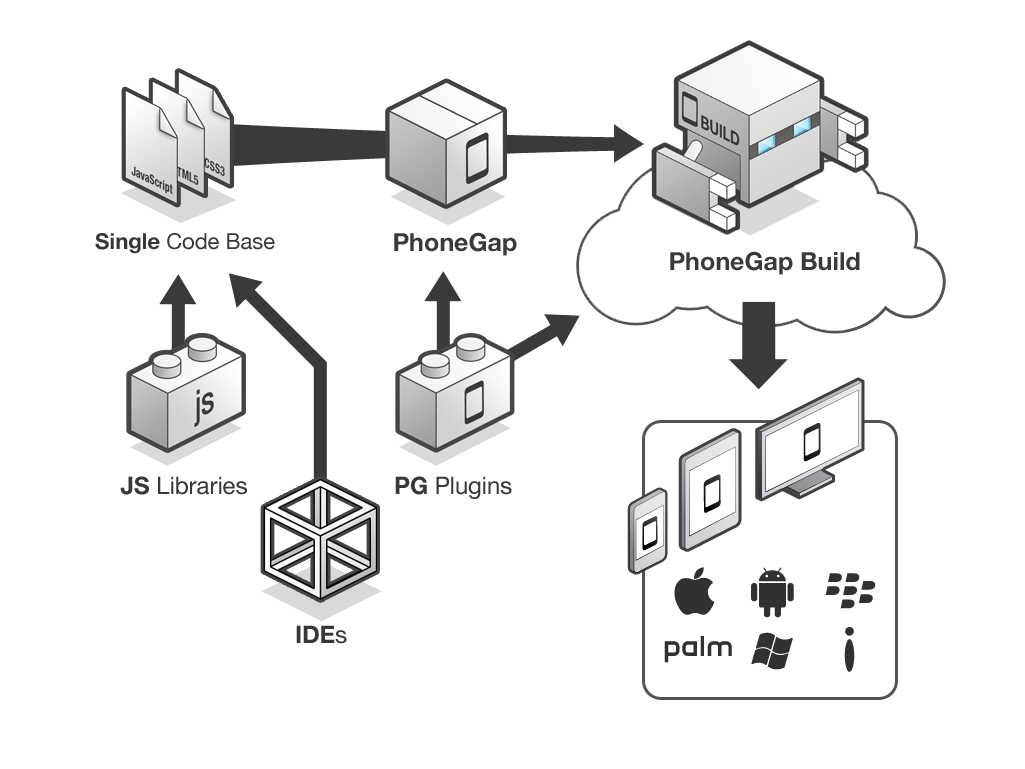
\includegraphics[width=.8\textwidth]{figs/cordova-architecture.png}
        \caption{The architecture of Apache Cordova/Adobe PhoneGap applications.}
        \label{fig:cordova:architecture}
    \end{center}
\end{figure}

One of Cordova's goals is to promote the web as a first-class development platform. However, many mobile browser implementations are still lacking decent HTML5 support. Cordova solves this problem by providing HTML5 polyfills for these browsers. A polyfill is a sort of plugins that addresses the lack of a specific feature in a browser. The API of the polyfill typically matches the official API such that applications do not notice that the feature is missing. If the browser does have support for a particular feature, the browsers implementation is used. 

\paragraph{Example} The Cordova Storage API is a polyfill for the deprecated but often used Web SQL specification\footnote{\url{http://dev.w3.org/html5/webdatabase/}} and Web Storage specification\footnote{\url{http://dev.w3.org/html5/webstorage/}}. 

Cordova has a pluggable architecture, i.e. within Cordova, every device API is implemented as a plugin. This allows to (1) leave out unused device API's, reducing the size of the compiled application and (2) create your own custom plugin. Every plugin comprises of a piece of JavaScript code and a piece of native code. Calls to the JavaScript API are marshaled and sent to the native counterpart where the request gets unmarshaled and executed. Additionally, a response is be sent back to the caller.

A comprehensive list of Cordova plugins is available at \url{https://github.com/phonegap/phonegap-plugins}. However, at the time of writing, there is no package manager like \texttt{npm}\footnote{NPM is the Node Package Manager, \url{http://npmjs.org}} available for Cordova plugins.

\subsection{Related projects}

There are a number of projects related to Apache Cordova that are useful when developing mobile web applications with Cordova.

\subsubsection{Adobe PhoneGap Build}

Adobe PhoneGap Build\footnote{\url{http://build.phonegap.com}}, part of Adobe Edge Tools \& Services, is an online build service for packaging Cordova/PhoneGap applications. Upon request, the application's source code is pulled from a git\footnote{Git is a popular version control system, \url{http://git-scm.org}} repository and the packaged app can be downloaded straight from the web interface. An API is available to automate the process. The service supports Android, iOS, Windows Phone, BlackBerry, WebOS and Symbian.

Both free and paid plans (with a monthly subscription fee) are available. The free plan is entitled to only one private project, a paid plan is entitled to 25 or more private apps.

\subsubsection{Edge Inspect}

Another Adobe product is called Edge Inspect\footnote{\url{http://html.adobe.com/edge/inspect/}}, which is also part of Adobe Edge Tools \& Services. It comprises of a desktop application, a Chrome plugin and a couple of native applications and allows developers to preview web designs on multiple displays at a time. When the plugin is activated, all connected devices instantly load the same web page. At the same time, developers get access to a WebKit inspector, showing the code of any remote browser (this is based on WEINRE, see further). The application also allows the developer to take screen shots the web pages displayed in a particular browser.

\subsubsection{WEINRE}

WEINRE\footnote{\url{http://people.apache.org/~pmuellr/weinre/docs/latest/}} is part of Apache Cordova and is an acronym for ``WEb INspector REmote''. It provides access to a fully functional WebKit inspector of remote browsers. The service runs on a node\footnote{Server-side JavaScript, \url{http://nodejs.org}} server. The only requirement is to include a javascript file in the application's HTML. When the browser starts executing the JavaScript file, it makes a persistent connection with a server through a web socket. This connection is then used for all communication between the web application and the WebKit inspector. This allows developers to inspect the DOM, resources, run custom JavaScript commands, etc. remotely.

A hosted version is available at \url{http://debug.phonegap.com}.

\subsubsection{Apache Ripple}

Apache Ripple\footnote{\url{http://ripple.incubator.apache.org}} is a web-based mobile environment simulator and is available as a Chrome extension. It exposes the Apache Cordova device API's and allows developers to simulate various device features in a desktop browser. For instance, you can shake the device, set a location and heading, emulate disruptive networking, etc.

\subsection{Proof-of-concept application implementation}

This subsection provides an overview and short description of the technologies that were used to implement the proof-of-concept application. 

The proof-of concept application is implemented as a single-page application. This eliminates page loads and thus improves overall performance of the application. The application code is all wrapped inside the native shell. Instead, future versions could serve application code from a remote server and use AppCache to cache the application data on the device. This way, the application can receive updates without the need of updating the outer shell. The application logic is built with AngularJS, the user interface is built on top of Bootstrap 3. The development workflow is based on Yeoman, which provides useful tools for scaffolding, building, previewing, testing, etc. Unit and integration tests are created with the Jasmine test framework and run with the Karma test runner.

\subsubsection{AngularJS}

AngularJS\footnote{\url{http://angularjs.org}} is an JavaScript MVC application framework, developed at Google. With AngularJS, developers can use a declarative programming style rather than an imperative style. This is achieved through additional HTML elements and attributes, which serve as annotations. In addition, the imperative programming style is still available to program controller code. AngularJS also provides a dependency injection system which makes testing so much easier. Components that require user interaction or are not useful in a testing environment can easily be replaced with a mock.

AngularJS has proven useful from the start. The project came to live at Google because developers of the Google Feedback project were unsatisfied with the development speed. The project that already took 6 months to create and 1700 lines of traditional HTML and JavaScript could be completely rewritten in three weeks by a single individual and with only 1500 lines of code \cite{Green:2013}.

\subsubsection{Bootstrap 3}

Bootstrap\footnote{\url{http://getbootstrap.com}} is a popular html user interface framework. Version 3 is a complete overhaul of the project, introducing a mobile-first approach. Instead of scaling down desktop pages, the new version starts from the mobile interface and scales up as the screen size increases. 

\subsubsection{Yeoman}

Yeoman\footnote{\url{http://yeoman.io}} is a collection of tools and best practices to make web development easier. It is comprised of the following tools:
\begin{itemize}
    \item \textbf{Yo} This command-line tool is used for scaffolding application code. A Yo plugin for AngularJS projects is available at \url{https://github.com/yeoman/generator-angular} and can generate various application artifacts.
    \item \textbf{Grunt} This command-line tool is similar to make\footnote{\url{https://www.gnu.org/software/make/}} and runs various predefined JavaScript tasks like compiling LESS files, minifying javascript and CSS, linting Javascript, running unit tests, etc.
    \item \textbf{Bower} This command-line tool is a package manager for web applications and takes care of hard to track dependencies in complex projects. 
\end{itemize}

\subsubsection{Jasmine \& Karma}

One of AngularJS' focal points is writing testable code. The community has created a test runner, called Karma\footnote{\url{http://karma-runner.github.io/}}. Running Karma will start a basic server, open a collection of browser windows (even mobile browser on connected devices or a headless browser like PhantomJS\footnote{\url{http://phantomjs.org/}}) and run all the tests in these browsers. The results of the tests are then passed back to the test runner in order to report them to the user. 

The tests are coded with the Jasmine\footnote{\url{http://pivotal.github.io/jasmine/}} testing framework.

\section{Motorola Rhodes}

\subsection{General information \& history}

Rhodes\footnote{\url{http://docs.rhomobile.com}} was developed and released in 2008 by an American company called RhoMobile. Their goal was to enable developers to quickly create native applications for all smartphones. Rhodes applications make use of synchronized local data and take advantage of the device's hardware. With a local synchronization engine, called RhoSync, the emphasis is clearly on data-driven enterprise applications.

In July 2011, Motorola Solutions (the non-mobile, enterprise and government-oriented division, not the division that was acquired by Google) acquired RhoMobile. After the acquisition, Motorola introduced the commercial product RhoElements: a set of specialized features like a barcode scanner, NFC and signature capture. About one year after the acquisition, Motorola removed a lot of the features from the Rhodes framework and included them in RhoElements version 2.

The Rhodes framework is open source and freely available under the MIT license. Based on the statistics of the RhoMobile Google groups page,  community activity has significantly decreased in the last year from 722 monthly posts in June 2012 to 102 monthly posts in April 2013. However, based on the contribution history on GitHub, development activity seems to have increased since January 2013.

\subsection{Supported platforms}

Rhodes currently supports all major platforms, including Android (2.1 and up), iOS (3.0 and up), Windows Phone 8 and BlackBerry (4, 5, 6 and 7).

\subsection{Architecture}

Rhodes is a cross-platform tool that creates applications that are both interpreted and hybrid at the same time. A Rhodes application is a mobile web application that runs locally on top of a Ruby web server, i.e. the application code it written in Ruby, the view is written in HTML. The architecture is depicted in \fref{fig:rhodes-architecture}.

\begin{figure}[h]
    \begin{center}
        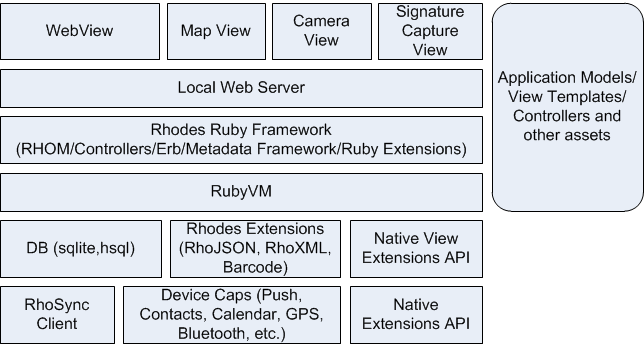
\includegraphics[width=0.9\textwidth]{figs/rhodes-architecture.png}
        \caption{The architecture of Rhodes applications}
        \label{fig:rhodes-architecture}
    \end{center}
\end{figure}

Rhodes also has a plugin system that allows developers to create native extensions for missing functionality. A plugin consists of a shared Ruby interface definition and native implementations for the supported platforms.

\subsection{Related projects}

Rhodes is an open-source framework is part of a collection of software, called RhoMobile Suite, which also contains other software products that fit strategically in this suite. These products are discussed briefly in this section.

\subsubsection{RhoElements}

RhoElements is a commercial product in the RhoMobile Suite and therefore requires a license. It contains a substantial amount of additional functionality that is useful for enterprise applications like NFC, barcode readers, etc. This functionality was removed from Rhodes in version 3.3.3.

\subsubsection{RhoConnect}

RhoConnect is another open-source product in the RhoMobile Suite and serves as a mobile orchestrator. It takes care of data synchronization between backend applications and mobile devices. The libraries for this integration are already available in the Rhodes framework.

\subsubsection{RhoHub}

RhoHub\footnote{\url{https://app.rhohub.com/}} is a cloud platform that developers can use to host and build their applications. Developers can push their code to a private git repository from which the application can be built for Android, iOS, etc.

\subsubsection{RhoStudio}

RhoStudio is an Ruby IDE, based on Eclipse 3.7, and contains a custom plugin for Rhodes and RhoElements application development. It is freely available as part of the RhoMobile Suite.

\subsection{Proof-of-concept application implementation}

The development of the proof-of-concept application was aborted early because the tooling was bugged and the performance of the resulting Rhodes applications was unsatisfying. On an entry-level smartphone, loading a page took 30 seconds and on a high-end smartphone page loads still take 7 seconds. Capgemini deemed this unacceptable and Rhodes was no longer considered a viable alternative.
\chapter{Evaluation}
\label{chap:evaluation}

This chapter presents a detailed description of the evaluation of the alternatives, which are the combination of native Android and native iOS, Apache Cordova and Motorola Rhodes. The chapter is structured as outlined in section \ref{sec:evaluation-method}: first, the weights of the criteria are calculated; second, the weights of the alternatives are calculate and last, a cost-benefit analysis is performed.

\section{Weighting the evaluation criteria}

Because developers and architects do not necessarily share the same opinions about the evaluation criteria, the ranking of the alternatives could be different as well. Therefore, this evaluation covers these two perspectives separately and the results for both perspectives are compared in the end. Both the developer and the architect were asked to fill in a questionnaire containing all necessary pairwise comparisons (see Appendix \ref{app:questionnaire}). 

The questioned people are the same people from the interviews earlier (see section \ref{sec:interviews}) and the results of the questionnaire are illustrated in \tref{tab:l1}, \tref{tab:portability}, \tref{tab:ae}, \tref{tab:productivity}, \tref{tab:ni}, \tref{tab:ui}.

\begin{table}[h!]
    \begin{center}
        \begin{tabular}{lcccl}
            \hline
            \textbf{Architect}     & Portability & App. Experience & Productivity & Priority vector \\ 
            \hline
            Portability            & $1$         & $1/3$           & $1/5$        & $0.1047$        \\
            App. Experience        & $3$         & $1$             & $5$          & $0.6370$        \\
            Productivity           & $5$         & $1/5$           & $1$          & $0.2583$        \\
            \hline
            \multicolumn{5}{r}{$\lambda_{max} = 3.5206$, $CI = 0.2603$, $RI = 0.58$, $CR = 0.4488$} \\
            \hline
        \end{tabular}
        \\\vspace{1em}
        \begin{tabular}{lcccl}
            \hline
            \textbf{Developer}     & Portability & App. Experience & Productivity & Priority vector \\ 
            \hline
            Portability            & $1$         & $1/7$           & $1/5$        & $0.0719$        \\
            App. Experience        & $7$         & $1$             & $3$          & $0.6491$        \\
            Productivity           & $5$         & $1/3$           & $1$          & $0.2790$        \\
            \hline
            \multicolumn{5}{r}{$\lambda_{max} = 3.0649$, $CI = 0.0324$, $RI = 0.58$, $CR = 0.0559$} \\
            \hline
        \end{tabular}
        \caption{Pairwise comparison matrix for the top level of the decision tree.}
        \label{tab:l1}
    \end{center}
\end{table}

The weights for the top level criteria are virtually the same for both the architect and the developer perspective. \tref{tab:portability} also reveals a high inconsistency in the architect's judgement ($CR > 0.1$). Analysis of the judgements shows that there is no loop, i.e. there is no chain $A, B, C$ such that $A$ is more important than $B$, $B$ is more important than $C$ and $C$ is more important than $A$. However, the judgement of portability vs. application experience does not reflect the judgement of application experience vs. productivity and the judgement of productivity vs. portability since $1/3 \not = 1/5 \times 1/5$. The inconsistency ratio for the judgement of the developer is acceptable as it is below 10\%.

\TODO{Ask for a better judgement?}

\begin{table}[h!]
    \begin{center}
        \begin{tabular}{lcccl}
            \hline
            \textbf{Architect}     & Platform support & Toolset reuse & Code reuse & Priority vector \\ 
            \hline
            Platform support         & $1$            & $1/3$         & $1/7$      & $0.0918$        \\
            Toolset reuse          & $3$            & $1$           & $5$        & $0.6248$        \\
            Code reuse             & $7$            & $1/5$         & $1$        & $0.2834$        \\
            \hline
            \multicolumn{5}{r}{$\lambda_{max} = 3.7089$, $CI = 0.2545$, $RI = 0.58$, $CR = 0.6112$}\\
            \hline
        \end{tabular}
        \\\vspace{1em}
        \begin{tabular}{lcccl}
            \hline
            \textbf{Developer}     & Platform support & Toolset reuse & Code reuse & Priority vector \\ 
            \hline
            Platform support         & $1$            & $1/5$         & $1/5$      & $0.0909\ldots$  \\
            Toolset reuse          & $5$            & $1$           & $1$        & $0.4545\ldots$  \\
            Code reuse             & $5$            & $1$           & $1$        & $0.4545\ldots$  \\
            \hline
            \multicolumn{5}{r}{$\lambda_{max} = 3$, $CI = 0$, $RI = 0.58$, $CR = 0$}               \\
            \hline
        \end{tabular}
        \caption{Pairwise comparison matrix for the category ``portability''.}
        \label{tab:portability}
    \end{center}
\end{table}

In the portability category (see \tref{tab:portability}), the differences between developer and architect are more pronounced. Just like before, the judgement of the architect shows a notable amount of inconsistency. Again, there is no loop but the comparison data violates the consistency property.

\TODO{Ask for better judgement?}

\begin{table}[h!]
    \begin{center}
        \begin{tabular}{lcccl}
            \hline
            \textbf{Architect}     & Native int. & UI capabilities & Performance & Priority vector \\ 
            \hline
            Native int.            & $1$         & $1$             & $3$         & $0.4600$        \\
            UI capabilities        & $1$         & $1$             & $1/3$       & $0.2211$        \\
            Performance            & $1/3$       & $3$             & $1$         & $0.3189$        \\
            \hline
            \multicolumn{5}{r}{$\lambda_{max} = 3.5608$, $CI = 0.2804$, $RI = 0.58$, $CR = 0.4835$}\\
            \hline
        \end{tabular}
        \\\vspace{1em}
        \begin{tabular}{lcccl}
            \hline
            \textbf{Developer}     & Native int. & UI capabilities & Performance & Priority vector \\ 
            \hline
            Native int.            & $1$         & $1$             & $1/5$       & $0.1428$        \\
            UI capabilities        & $1$         & $1$             & $1/5$       & $0.1428$        \\
            Performance            & $5$         & $5$             & $1$         & $0.7142$        \\
            \hline
            \multicolumn{5}{r}{$\lambda_{max} = 3$, $CI = 0$, $RI = 0.58$, $CR = 0$}               \\
            \hline
        \end{tabular}
        \caption{Pairwise comparison matrix for the category ``Application Experience''.}
        \label{tab:ae}
    \end{center}
\end{table}

\begin{table}[h!]
    \begin{center}
        \begin{tabular}{lccl}
            \hline
            \textbf{Architect}     & Access to HW & Platform-specific svc. & Priority vector \\
            \hline
            Access to HW           & $1$          & $1/3$                  & $0.2500$        \\
            Platform-specific svc. & $3$          & $1$                    & $0.7500$        \\
            \hline
            \multicolumn{4}{r}{$\lambda_{max} = 2$, $CI = 0$, $RI = 0$, $CR = 0$}            \\
            \hline
        \end{tabular}
        \\\vspace{1em}
        \begin{tabular}{lccl}
            \hline
            \textbf{Developer}     & Access to HW & Platform-specific svc. & Priority vector \\
            \hline
            Access to HW           & $1$          & $5$                    & $0.8333\ldots$  \\
            Platform-specific svc. & $1/5$        & $1$                    & $0.1666\ldots$  \\
            \hline
            \multicolumn{4}{r}{$\lambda_{max} = 2$, $CI = 0$, $RI = 0$, $CR = 0$}            \\
            \hline
        \end{tabular}
        \caption{Pairwise comparison matrix for the category ``Native integration'' within the category ``Application Experience''.}
        \label{tab:ni}
    \end{center}
\end{table}

\begin{table}[h!]
    \begin{center}
        \begin{tabular}{lccl}
            \hline
            \textbf{Architect}  & Native L\& F & UI el. capabilities & Priority vector \\
            \hline
            Native L\& F        & $1$          & $5$                 & $0.8333\ldots$  \\
            UI el. capabilities & $1/5$        & $1$                 & $0.1666\ldots$  \\
            \hline
            \multicolumn{4}{r}{$\lambda_{max} = 2$, $CI = 0$, $RI = 0$, $CR = 0$}      \\
            \hline
        \end{tabular}
        \\\vspace{1em}
        \begin{tabular}{lccl}
            \hline
            \textbf{Developer}  & Native L\& F & UI el. capabilities & Priority vector \\
            \hline
            Native L\& F        & $1$          & $1/5$               & $0.1666\ldots$  \\
            UI el. capabilities & $5$          & $1$                 & $0.8333\ldots$  \\
            \hline
            \multicolumn{4}{r}{$\lambda_{max} = 2$, $CI = 0$, $RI = 0$, $CR = 0$}      \\
            \hline
        \end{tabular}
        \caption{Pairwise comparison matrix for the category ``UI capabilities'' within the category ``Application Experience''.}
        \label{tab:ui}
    \end{center}
\end{table}

\begin{table}[h!]
    \begin{center}
        \begin{tabular}{lcccl}
            \hline
            \textbf{Architect} & Skill reuse & Tooling & Testing & Priority vector \\
            \hline
            Skill reuse        & $1$         & $1/5$   & $3$     & $0.2021$        \\
            Tooling            & $5$         & $1$     & $5$     & $0.7007$        \\
            Testing            & $1/3$       & $1/5$   & $1$     & $0.0972$        \\
            \hline
            \multicolumn{5}{r}{$\lambda_{max} = 3.1356$, $CI = 0.0678$, $RI = 0.58$, $CR = 0.1169$}\\
            \hline
        \end{tabular}
        \\\vspace{1em}
        \begin{tabular}{lcccl}
            \hline
            \textbf{Developer} & Skill reuse & Tooling & Testing & Priority vector \\
            \hline
            Skill reuse        & $1$         & $1$     & $3$     & $0.4286$        \\
            Tooling            & $1$         & $1$     & $3$     & $0.4286$        \\
            Testing            & $1/3$       & $1/3$   & $1$     & $0.1428$        \\
            \hline
            \multicolumn{5}{r}{$\lambda_{max} = 3$, $CI = 0$, $RI = 0.58$, $CR = 0$}               \\
            \hline
        \end{tabular}
        \caption{Pairwise comparison matrix for the category ``Productivity''.}
        \label{tab:productivity}
    \end{center}
\end{table}




\section{Evaluate the alternatives}

In the following subsections, all alternatives get evaluated with respect to one criterion at a time. Every subsection provides a description of what is measured and how, what is taken into account for the evaluation and what scale is used and why. For every alternative, the rationale for the judgement or score will be provided as well.

In case judgements are used, these judgements are based on the experience of developing the proof-of-concept application. Some criteria discuss features that are not part of the proof-of-concept application. In that case, the information is taken from the documentation. 

\subsection{Platform support}

Remember from section \ref{sec:selection-criteria} that support for Android and iOS is a selection criterion. This criterion only covers additional platforms, apart from Android and iOS. To reflect the value of each platform, every alternative is awarded the additional market share it can serve. In the end, these scores are normalized such that the sum of scores is equal to 1. The market share numbers are taken from \fref{fig:smartphone-share}.

\paragraph{Android \& iOS} Native code for Android and iOS is useless on other platforms. Hence, the combination of Android and iOS cannot contribute to reaching additional market share.

\paragraph{Apache Cordova} From Cordova's platform support (see section \ref{sec:ac:support}), it is safe to say that it supports the remainder of the mobile market. Cordova is therefore awarded the remaining 17\% of market share: 6\% for BlackBerry, 6\% for Symbian, 2\% for Windows Phone, 2\% for Bada and 1\% for the remainder of mobile platforms.

\paragraph{Motorola Rhodes} Rhodes only supports BlackBerry and Windows Phone for which it is awarded 8\% of market share: 6\% for BlackBerry and 2\% for Windows Phone. 

\paragraph{Verdict} The normalized scores are listed in \tref{tab:ps}. 

\begin{table}[h!]
    \begin{center}
        \begin{tabular}{lcccl}
            \hline
            \textbf{Platform support} & Market share & Normalized weight \\
            \hline
            Android/iOS               & $0\%$        & $0$         \\
            Cordova                   & $17\%$       & $0.68$      \\
            Rhodes                    & $8\%$        & $0.32$      \\
            \hline
        \end{tabular}
        \caption{Evaluation of the alternatives with respect to ``platform support''.}
        \label{tab:ps}
    \end{center}
\end{table}

\subsection{Toolset reuse}

This criterion describes the ability to reuse the development environment or parts thereof when migrating to another cross-platform alternative. The evaluation is based on the recommended development environment setup for each alternative. Since there is no absolute scale available to measure this property, Saaty's fundamental scale (see \tref{tab:ahp-scale}) is used here.

\paragraph{Android \& iOS} All iOS development is done with the Xcode IDE, which is available on Apple computers only. Every iOS developer must therefore have a rather expensive Mac. For Android development, any platform can be used in combination with the Android SDK and an Eclipse plugin (ADT) is available. On I/O 2013, Google also announced a new, freely available Android IDE, based on JetBrains' IntelliJ.

\paragraph{Apache Cordova} For HTML5 application development, any operating system with a web IDE or even a simple text editor will do. However, packaging the Cordova application in its native shell requires the native SDK's or the online build service, called PhoneGap Build, provided by Adobe. Unfortunately, this service cannot build additional plugins that are not part of the standard distribution. If a project makes use of custom plugins, the native SDK's are required. 

\paragraph{Motorola Rhodes} Development of Rhodes applications requires a Ruby installation and a Ruby IDE. A specially tailored Eclipse-based Ruby IDE, called RhoStudio, is distributed as part of RhoMobile. As with Cordova, packaging the app requires the native SDK or the online build service, called RhoHub, provided by Motorola.

\paragraph{Verdict} Motorola Rhodes and Apache Cordova have similar requirements and therefore they are treated equally in the comparison. 
Native development for Android and iOS is treated as a whole. Because of the strict requirements imposed by Apple, native development scores a little less compared to Cordova and Rhodes. However, not being able to build the application locally is not very practical either, which explains the scores listed in \tref{tab:tr}.

\begin{table}[h!]
    \begin{center}
        \begin{tabular}{lcccl}
            \hline
            \textbf{Toolset reuse} & Android/iOS & Cordova & Rhodes & Priority vector \\
            \hline
            Android/iOS            & $1$         & $1/3$   & $1/3$  & $0.1428$        \\
            Cordova                & $3$         & $1$     & $1$    & $0.4286$        \\
            Rhodes                 & $3$         & $1$     & $1$    & $0.4286$        \\
            \hline
            \multicolumn{5}{r}{$\lambda_{max} = 3$, $CI = 0$, $RI = 0.58$, $CR = 0$}  \\
            \hline
        \end{tabular}
        \caption{Evaluation of the alternatives with respect to ``toolset reuse''.}
        \label{tab:tr}
    \end{center}
\end{table}

\subsection{Code reuse}

This criterion measures the amount of code that can be reused when migrating to another platform. For this criterion, the amount of portable code is expressed as an estimated percentage of the total amount of application code. Native extensions are not taken into account as they are not part of the application logic. They are considered to be reusable dependency which has to be coded once. 

\paragraph{Android \& iOS} As mentioned before, native code for Android and iOS is useless on other platforms but native Android code is also useless on iOS and vice versa. Hence, code reuse on Android and iOS is 0\%.

\paragraph{Apache Cordova} Code reuse is 100\% for Cordova applications because all code is shared across all platforms. Since code of native plugins are not taken into account, this does not affect the score.

Note that a large amount of code can potentially be reused in other (non-mobile) platforms. Be that as it may, it is out of the scope of this evaluation and it is not taken into account either.

\paragraph{Motorola Rhodes} Code reuse on Rhodes applications is also 100\%. It is not taken into account that Rhodes has no support for custom plugins and that its code is not as widely deployable.

\paragraph{Verdict} The scores for each alternative are normalized and listed in \tref{tab:cr}. 

\begin{table}[h!]
    \begin{center}
        \begin{tabular}{lcccl}
            \hline
            \textbf{Toolset reuse} & Code reuse & Priority vector \\
            \hline
            Android/iOS            & $0\%$       & $0$            \\
            Cordova                & $100\%$     & $0.5000$       \\
            Rhodes                 & $100\%$     & $0.5000$       \\
            \hline
        \end{tabular}
        \caption{Evaluation of the alternatives with respect to ``code reuse''.}
        \label{tab:cr}
    \end{center}
\end{table}

\subsection{Access to hardware}

This criterion measures the ability to integrate the device's hardware. For this criterion, the availability of device API's (sensor API's, output API's and communication API's) is studied and every alternative is awarded the fraction of device API's it supports. Alternatives can either provide full support (there is a way to access a particular piece of hardware or software on both platforms), partial support (access to this type of hardware is available on one platform only) or no support. Note that most of these API's are not used in the proof-of-concept application. Therefore, this comparison is mostly based on the documentation of the alternatives.

\paragraph{Android \& iOS} Android provides support for all types of sensors but that does not imply that all these sensors are available in a particular device. Apple iDevices have less sensors and as such there is no support for every sensor in iOS.

\paragraph{Apache Cordova} Cordova tries to promote the web as a first-class platform for mobile applications. ``The ultimate purpose of \emph{Cordova} is to cease to exist'' \cite{LeRoux:2012}. When HTML5 will be fully supported on all mobile browsers, Cordova will no longer be needed. Therefore, all Cordova API's (try to) follow the HTML5 specification and do not provide support for all the sensors and communication because they are simply not in the specification.

Note that with Cordova's plugin system, it can deliver the same level of integration as native Android and iOS. However, the plugin system is not taken into account here. 

\paragraph{Motorola Rhodes} Rhodes provides a reasonable amount device API's. All of them are available through ruby method calls. As of version 3.3.3, Motorola has removed a lot of API's and included them in their commercial product called RhoMobile Suite, for which additional API's are available.

\paragraph{Verdict} The studied device API's and the alternative's support for it are listed in \tref{tab:apis}.

\begin{table}[h]
    \begin{center}
        \begin{tabular}{lcccc}
            \hline
            API                 & Android        & iOS        & Cordova    & Rhodes     \\
            \hline
            Accelerometer       & \checkmark     & \checkmark & \checkmark & \checkmark \\
            Geolocation         & \checkmark     & \checkmark & \checkmark & \checkmark \\
            Gyroscope           & \checkmark     & \checkmark & --         & \checkmark \\
            Light               & \checkmark     & \checkmark & --         & \checkmark \\
            Magnetic Field      & \checkmark     & \checkmark & \checkmark & \checkmark \\
            Pressure            & \checkmark     & --         & --         & partial    \\
            Proximity           & \checkmark     & \checkmark & --         & \checkmark \\
            Relative Humidity   & \checkmark     & --         & --         & partial    \\
            Temperature         & \checkmark     & --         & --         & partial    \\
            Microphone          & \checkmark     & \checkmark & \checkmark & \checkmark \\
            Camera              & \checkmark     & \checkmark & \checkmark & \checkmark \\
            Hardware buttons    & \checkmark     & --         & partial    & partial    \\
            Vibration Motor     & \checkmark     & \checkmark & \checkmark & partial    \\
            Speaker             & \checkmark     & \checkmark & \checkmark & \checkmark \\
            System information  & \checkmark     & \checkmark & \checkmark & \checkmark \\
            File System         & \checkmark     & \checkmark & \checkmark & \checkmark \\
            Contacts            & \checkmark     & \checkmark & \checkmark & \checkmark \\
            Bluetooth           & \checkmark     & \checkmark & --         & \checkmark \\
            NFC                 & \checkmark     & --         & --         & --         \\
            Wi-Fi Direct        & \checkmark     & --         & --         & --         \\
            USB / Accessory     & \checkmark     & \checkmark & --         & --         \\
            \hline
            Support             & \multicolumn{2}{c}{$18/21$} & $10.5/21$  & $15.5/21$  \\
            \hline
        \end{tabular}
        \caption{}
        \label{tab:apis}
    \end{center}
\end{table}

\subsection{Integration with platform-specific services}
\TODO{Drop this comparison? Not really identifiable from the interviews or literature... and kind of based on nothing :/}

This criterion measures the ability to integrate the application with platform-specific services that might not be available on all platforms. Again, because there is no absolute scale to express this ability, Saaty's fundamental scale is used.

\paragraph{Android \& iOS} The native SDK's are best suited for this kind of integration. 

\paragraph{Apache Cordova} There are no API's for this kind of integration in the default Cordova distribution. Nevertheless, one can integrate rather easily with these services through a custom plugin.

\paragraph{Motorola Rhodes} There are no API's for this integration in Rhodes either. Moreover, Rhodes does not have a plugin system which could make this integration possible. Therefore, it is excluded from this category and not awarded any points.

\paragraph{Verdict} The scores are listed in \tref{tab:pss}. Integrating with platform specific services is clearly more easy with the native development kits.

\begin{table}[h!]
    \begin{center}
        \begin{tabular}{lcccl}
            \hline
            \textbf{Performance} & Android/iOS & Cordova & Rhodes & Priority vector \\
            \hline
            Android/iOS          & $1$         & $5$     & excl. & $0.8333\ldots$        \\
            Cordova              & $1/5$       & $1$     & excl. & $0.1667\ldots$        \\
            Rhodes               & excl.       & excl.   & excl. & $0$        \\
            \hline
            \multicolumn{5}{r}{$\lambda_{max} = 2$, $CI = 0$, $RI = 0$, $CR = 0$}\\
            \hline
        \end{tabular}
        \caption{Evaluation of the alternatives with respect to ``platform-specific services''}
        \label{tab:pss}
    \end{center}
\end{table}

\subsection{Native Look \& Feel}

This criterion indicates whether or not an alternative is able to use native user interface elements. An application can either support the use of native user interface elements fully, partially or not at all.

\paragraph{Android \& iOS} It needs no explaining that Android and iOS can use the native user interface elements.

\paragraph{Apache Cordova} The user interface of Cordova applications is built with HTML5, CSS and JavaScript and there is no possibility to use native user interface elements for it. 

However, numerous attempts are made to recreate the native look \& feel on top of HTML (like KendoUI, Moobile, etc.). Unfortunately, these projects need a lot of additional code to mimic the behaviour of native interface elements which influences the overall performance of the application in a adverse way.

\paragraph{Motorola Rhodes} The user interface of Rhodes applications is also built with HTML and consequently cannot deliver the native look \& feel to the end user.

\paragraph{Verdict} Despite the efforts of many projects to mock the native look \& feel in web applications, it remains a privilege of Android and iOS. Hence, Android and iOS clearly do better compared to Cordova and Rhodes, as is illustrated in \tref{tab:nlf}.

%\begin{table}[h!]
%    \begin{center}
%        \begin{tabular}{lcl}
%            \hline
%            \textbf{Native Look \& Feel} & Able to use native UI elements & Priority vector \\
%            \hline
%            Android/iOS          & Yes          & $1$        \\
%            Cordova              & No       & $1$     & $1$   & $0.0909\ldots$        \\
%            Rhodes               & No       & $1$     & $1$   & $0.0909\ldots$        \\
%            \hline
%        \end{tabular}
%        \caption{Pairwise comparison matrix for the criterion ``Native Look \& Feel''.}
%        \label{tab:nlf}
%    \end{center}
%\end{table}

\subsection{UI element capabilities}

This criterion measures an alternative's potential to present a rich user interface. Both Cordova and Rhodes rely on HTML for their user interface. Therefore, the evaluation is based on a comparison of the native UI elements with their HTML5 counterparts. Plain HTML only provides basic interface elements, which is why an additional UI framework, called Bootstrap\footnote{\url{http://getbootstrap.com}}, was used to develop the proof-of-concept application. 

\paragraph{Android \& iOS} Android and iOS both have an elaborate portfolio of rich user interface elements. iOS lacks some basic form elements like radio buttons and checkboxes but these can be easily replaced with pickers and switches respectively.

\paragraph{Apache Cordova} Cordova applications are mobile web applications that are wrapped in a single webview. Hence, only HTML5 can be used to create the user interface. An application could be comprised of multiple pages or it could be comprised of a single page, in which case it is called  a single-page application. The former approach requires page reloads, which feels unnatural in a mobile app (compared to native apps) whereas the latter approach can make the hybrid app behave more like a native app. 

The Cordova proof-of-concept application is implemented as a single-page application with AngularJS\footnote{\url{http://angularjs.org}}. This framework drastically improves productivity by reducing the required lines of code through declarative programming and bidirectional bindings between view and model. 

\paragraph{Motorola Rhodes} Rhodes also relies on HTML for its user interface. In contrast to Cordova, Rhodes is actually a complete web server with an MVC framework on top. Every request is handled locally by a controller action and the result is served in a webview. Developers can still choose to create single-page applications but device integration has to be realized through AJAX\footnote{Asynchronous JavaScript and XML} calls, which requires extra work. The proof-of-concept application is implemented as a multi-page application because this is the default way to develop applications with Rhodes.

\paragraph{Verdict} The scores are listed in \tref{tab:uiec}.

\begin{table}[h]
    \begin{center}
        \begin{tabular}{llll}
            \hline
            Android         & iOS              & HTML5                          & Bootstrap 3             \\
            \hline
            ActionBar       & UINavigationBar  & --                             & \html{navbar} class     \\
            Split ActionBar & UIToolbar        & --                             & \html{navbar} class     \\
            Tabs            & UITabBar         & --                             & \html{nav-tabs} class   \\
            ListView        & UITableView      & --                             & \html{list-group} class \\
            GridList        & UICollectionView & --                             & Grid system             \\            
            ScrollView      & UIScrollView     & by default                     & --                      \\
            Spinner         & --               & \html{<select></select>}       & \html{dropdown} class   \\
            Picker          & UIPickerView     & \html{<select></select>}       & \html{modal} class      \\
            DatePicker      & UIDatePicker     & \html{<input type="date">}     & --                      \\
            Button          & UIButton         & \html{<button></button>}       & \html{btn} class        \\
            Text field      & UITextField      & \html{<input type="...">}      & --                      \\
            Slider          & UISlider         & \html{<input type="range">}    & --                      \\
            Progress bar    & UIProgressBar    & \html{<progress>}              & \html{progress} class   \\
            Options Menu    & UIActionSheet    & --                             & --                      \\
            Checkbox        & --               & \html{<input type="checkbox">} & --                      \\
            Radio           & --               & \html{<input type="radio">}    & --                      \\
            On/off switch   & UISwitch         & --                             & \html{btn-group} class  \\
            Dialog          & UIDialog         & --                             & \html{modal} class      \\
            Alert           & UIAlertView      & \html{alert(string)}           & --                      \\
            Popup           & --               & --                             & \html{modal} class      \\
            Toast           & --               & --                             & \html{alert} class      \\
            TextView        & UILabel          & any text element               & --                      \\
            MapView         & MKMapView        & --                             & --                      \\
            --              & Popover (iPad)   & --                             & \html{popover} script   \\
            Master-Detail   & SplitView (iPad) & --                             & Grid System             \\
            WebView         & UIWebView        & \html{<iframe>}                & --                      \\
            \hline
            \multicolumn{2}{c}{Android \& iOS combined: $26/26$} & \multicolumn{2}{c}{HTML5 \& Bootstrap combined: $24/26$}                 \\
            \hline
        \end{tabular}
        \caption{}
        \label{tab:uiec}
    \end{center}
\end{table}


\subsection{Performance}

The performance criterion measures the responsiveness of the user interface and the application in general. Responsiveness in this case does not mean the ability to reflow UI elements to fit other screen sizes, responsiveness in this case represents the time it takes an application to respond to a trigger, like pushing a button.

Comparing the performance of these alternatives is very hard because their architectures are so different. For instance, measuring page load times is impossible because the Rhodes application is the only application that uses page loads. There is no notion of a page load in native applications and the Cordova application is implemented as a single-page application. 

Fortunately, the analytic hierarchy process can make up for this because it inherently assumes error in human judgement. As long as the consistency ratio is low, the judgements are acceptable.

Every implementation of the proof-of-concept application is tested on four devices:
\begin{itemize}
    \item \textbf{HTC Wildfire S} An entry-level smartphone, released in May 2011 and running Android 2.3.5 on a single core 600\,MHz ARMv6 processor. It has 512\,MB of RAM and a 3.2-inch display with a 320 by 480 pixel resolution (180\,ppi).
    \item \textbf{HTC Flyer} An entry-level tablet, also released in May 2011 and running Android 3.2.2 on a single core 1.5\,GHz ARMv7 processor. It has 1024\,MB of RAM and a 7.0-inch display with a 600 by 1024 pixel resolution (170\,ppi).
    \item \textbf{LG/Google Nexus 4} A high-end smartphone, released in November 2012 and running Android 4.2.2 on a quad core 1.5\,GHz ARMv7 processor. It has 2048\,MB of RAM and a 4.7-inch display with a 768 by 1280 pixel resolution (318\,ppi).
    \item \textbf{iPhone 3GS} A smartphone, released in June 2009 and running iOS 6.1.3 on a single core 600\,MHz ARMv6 processor. It has 256\,MB of RAM and a 3.5-inch display with a 320 by 480 pixel resolution (165\,ppi).
\end{itemize}

\paragraph{Android \& iOS} \TODO{Best}

\paragraph{Apache Cordova} \TODO{average/worse than average}

\paragraph{Motorola Rhodes} \TODO{Worst}

\paragraph{Verdict} The final scores are listed in \tref{tab:performance}.

\begin{table}[h!]
    \begin{center}
        \begin{tabular}{lcccl}
            \hline
            \textbf{Performance} & Android/iOS & Cordova & Rhodes & Priority vector \\
            \hline
            Android/iOS          & $1$         & $5$     & $9$    & $0.7352$        \\
            Cordova              & $1/5$       & $1$     & $5$    & $0.2067$        \\
            Rhodes               & $1/9$       & $1/5$   & $1$    & $0.0581$        \\
            \hline
            \multicolumn{5}{r}{$\lambda_{max} = 3$, $CI = 0.0585$, $RI = 0.58$, $CR = 0.10$}\\
            \hline
        \end{tabular}
        \caption{Pairwise comparison matrix for the criterion ``Performance''.}
        \label{tab:performance}
    \end{center}
\end{table}

\subsection{Skill reuse}

This criterion expresses the ability to reuse skills from another field of expertise to develop mobile applications. This allows for better resource management. For this criterion, it is assumed that the organization has got a substantial expertise with Java EE (because Capgemini does). 

\paragraph{Android \& iOS} For organizations that already have got  expertise with Java EE applications, the entry barrier for adding Android to the portfolio is rather low, since Android is based on Java. Adding iOS from that perspective is less straightforward, because Objective-C is a new programming language.

\paragraph{Apache Cordova} In order to develop Cordova applications, one needs to know the web. Since the web already belongs to the organization's expertise, this skill can be reused quite easily but developers will probably have to invest in their JavaScript skills. When custom plugins are needed, the scenario of native Android and iOS holds.

\paragraph{Motorola Rhodes} For Rhodes applications, organizations can reuse their skills for creating the user interface. However, the application logic entirely written in Ruby, which is a new programming language for the organization.

\paragraph{Verdict} The native SDK's and Rhodes are similar because one needs to learn a new language for either of both. For the development of Cordova application, no notable new skills are required, explaining the scores listed in \tref{tab:sr}.

\TODO{On the other hand, learning Objective-C appeared to be easier than learning Ruby (in combination with Rhodes) when developing the proof-of-concept application. The free online video lectures about iOS development by Paul Hegarty are very valuable.}


\begin{table}[h!]
    \begin{center}
        \begin{tabular}{lcccl}
            \hline
            \textbf{Skill reuse} & Android/iOS & Cordova & Rhodes & Priority vector \\
            \hline
            Android/iOS          & $1$         & $1/5$   & $1/5$  & $0.1428$        \\
            Cordova              & $5$         & $1$     & $5$    & $0.7144$        \\
            Rhodes               & $1$         & $1/5$   & $1$    & $0.1428$        \\
            \hline
            \multicolumn{5}{r}{$\lambda_{max} = 3$, $CI = 0$, $RI = 0.58$, $CR = 0$}\\
            \hline
        \end{tabular}
        \caption{Pairwise comparison matrix for the criterion ``Skill reuse''.}
        \label{tab:sr}
    \end{center}
\end{table}

\subsection{Tooling}

This criterion describes the overall quality of the supplied tools. This includes command-line interfaces, IDE's, emulators and others. Since there is no absolute scale available to measure the quality accurately, the alternatives are compared in pairs. Saaty's scale is used to express the scores that are based on the experience of developing the proof-of-concept application.

\paragraph{Android \& iOS} The restrictions on Apple development may seem obstructive at first but it also allows Apple to deliver a well integrated development environment. Everything a developer could possibly need is available in Xcode, right out of the box. For Android development, an Eclipse plugin is available which integrates all the functionality of the SDK with the IDE. 

\paragraph{Apache Cordova} Cordova does not ship with an elaborate IDE or special development tools. However, there are some tools that can ease the development of mobile web applications (WEINRE, Ripple emulator, etc.). Unfortunately, there is no integrated development environment. 

\paragraph{Motorola Rhodes} Rhodes comes with a bunch of command-line scripts. Sadly, the Android Debug Bridge (ADB) is poorly integrated \TODO{(see section \ref{sec:mr:tools})} and there is no option to transfer iOS applications to an iDevice from the command-line interface. Instead, either Xcode, iTunes or Fruitstrap is needed for the transfer. 

\TODO{What about RhoStudio?}

\paragraph{Verdict} The scores about the quality of the tools are based on the experience from developing the proof-of-concept application and are listed in \tref{tab:tooling}. 

\begin{table}[h!]
    \begin{center}
        \begin{tabular}{lcccl}
            \hline
            \textbf{Tooling} & Android/iOS & Cordova & Rhodes & Priority vector \\
            \hline
            Android/iOS      & $1$         & $3$     & $9$    & $0.6716$        \\
            Cordova          & $1/3$       & $1$     & $5$    & $0.2654$        \\
            Rhodes           & $1/9$       & $1/5$   & $1$    & $0.0629$        \\
            \hline
            \multicolumn{5}{r}{$\lambda_{max} = 3$, $CI = 0.0145$, $RI = 0.58$, $CR = 0.025$}\\
            \hline
        \end{tabular}
        \caption{Pairwise comparison matrix for the criterion ``Tooling''.}
        \label{tab:tooling}
    \end{center}
\end{table}

\subsection{Testing}

The testing criterion measures the ability to automate testing and the ability to be used in a continuous integration environment. Again, Saaty's scale is used as there is no absolute scale available to measure this property. This criterion focusses mainly on unit testing and integration testing as these tests are ran the most in a continuous integration environment. Mobile interface testing is rather hard and is not taken into consideration for this criterion.

\paragraph{Android \& iOS} The programming language for native Android applications is Java and consequently, the well-known JUnit framework can be used for testing. A similar framework is readily available in Xcode for Objective-C.

\paragraph{Apache Cordova} \TODO{Test Runner Karma (formerly Testacular) + Test Framework Jasmine.}

Need some more research on this topic

\paragraph{Motorola Rhodes} \TODO{SpecRunner}

Need some more research on this topic

\paragraph{Verdict} The scores are listed in \tref{tab:testing}.

\begin{table}[h!]
    \begin{center}
        \begin{tabular}{lcccl}
            \hline
            \textbf{Testing} & Android/iOS & Cordova & Rhodes & Priority vector \\
            \hline
            Android/iOS      & $1$         & $1$     & $1$    & $0.3333\ldots$        \\
            Cordova          & $1$         & $1$     & $1$    & $0.3333\ldots$        \\
            Rhodes           & $1$         & $1$     & $1$    & $0.3333\ldots$        \\
            \hline
            \multicolumn{5}{r}{$\lambda_{max} = 3$, $CI = 0$, $RI = 0.58$, $CR = 0$}\\
            \hline
        \end{tabular}
        \caption{Pairwise comparison matrix for the criterion ``Testing''.}
        \label{tab:testing}
    \end{center}
\end{table}

\subsection*{Global verdict}




\section{Costs versus benefits}















\chapter{Conclusion}
\label{chap:conclusion}

This final chapter presents a summary of the work, together with a critical reflection and an overview of potential future improvements. 

\section{Goals}
\label{sec:goals}

This thesis had two major goals. The first goal was to design a methodology for evaluating and selecting a cross-platform tool for mobile application development. The second goal was to use this methodology to evaluate real cross-platform tools and select the most suited candidate. The methodology that was used is inspired by the generic software package selection, presented by \citet{Jadhav:2011}, and comprises of six highly customizable stages. Each of these stages has been concretized in Chapter \ref{chap:methodology}. 

During the first stage, the selection criteria were gathered. These are the most essential requirements that a cross-platform tools has to meet. The selection criteria were defined by Capgemini and require cross-platform tools to produce native applications for both Android and iOS and for both smartphones and tablets. 

During the second stage, a list of potential candidates was composed from Internet searches and literature. An extensive list of cross-platform tools was found in ``Cross-platform developer tools 2012'', a report by VisionMobile on this subject \cite{VMCPT:2012}. Subsequent Internet searches did not reveal new tools.

During the third stage, this list of potential candidates was filtered using the selection criteria from the first stage and from the resulting list, two cross-platform tools were selected for evaluation. These tools are Apache Cordova and Motorola Rhodes (see Chapter \ref{chap:tools}). The native development kits for both Android and iOS were also included as a baseline for the evaluation. 

During the fourth stage, the evaluation criteria were defined. Three people at Capgemini were interviewed: a developer, a mobile architect and a sales person. From these interviews and literature, eleven evaluation criteria were identified: platform support, toolset reuse, code reuse, access to hardware, integration with platform-specific services, native look \& feel, user interface capabilities, performance, skill reuse, tooling and testing. These criteria are organized in a hierarchy because humans can only process 7 plus or minus 2 pieces of information at the same time.

During the fifth stage, the alternatives were evaluated using these evaluation criteria. For this evaluation, the Analytic Hierarchy Process (AHP) \cite{Saaty:1980} was used. This method assigns weights to both criteria and alternatives based on judgements that originate from pairwise comparisons. In order to formulate a reliable judgement, a proof-of-concept application was implemented with the studied tools. The evaluation is carried out from two perspectives: one from the perspective of a developer, one of a perspective of a mobile architect. Both could have different opinions about cross-platform tool qualities, which could result in a different ranking.

During the sixth and last stage, the candidates that is are most suited were carefully selected. This required a cost-benefit analysis to ascertain that the selected alternative was also cost-effective. For this cost-benefit analysis, development time was used as a cost driver and the scores for the alternatives, obtained from the evaluation, were used as benefits. From this analysis, it was concluded that Apache Cordova is currently equally cost-effective as the native development kits when only targeting Android and iOS. However, if in the future a third platform has to be supported, Cordova will be more cost-effective because the application can be completely reused on the next platform.

\section{Reflection and future work}
\label{sec:reflection}

The methodology presented in this thesis ends with the selection of a cross-platform tool. However, the usefulness of this tool is never validated. Hence, a seventh, validation stage seems desirable. However, it is not possible to include this step in the timeframe of this thesis because such validation requires that the tool is used in a production environment for quite some time. The prolonged use of a particular tool in a large-scale environment will definitely reveal more benefits and/or issues than a simple proof-of-concept application can in a small-scale and controlled environment. Ergo, this seventh step is of utmost importance after the selection of a cross-platform tool.

Also, the mobile industry is rapidly evolving, which inherently makes cross-platform tools moving targets. The outcome of this study will probably be different in one year from the moment of writing. This makes continuous evaluation of the available tools a necessity and introduces a feedback loop in the evaluation process. New technologies often provide less functionality in the early stages of its life cycle but they can quickly overcome the functionality of the current technologies. New tools can be deemed ineffective at a certain time, but may become more effective than the current tools in the future. Frequent reevaluation is a must.

From the cost-benefit analysis in this study it is concluded that Apache Cordova and the native development kits are currently equally cost-effective. If a company decides to use Cordova for a number of its applications, a new problem rises because Cordova only wraps (mobile) web applications. There is a large number of tools available for (mobile) web development. Working with each of these technologies will create a different experience, both for developers and end-users, which motivates the need for another comparative study, a study that compares tools for (mobile) web development. 

During the evaluation phase, the criteria are weighted using the judgements of only two individuals. The evaluation is based on the judgement of the evaluator. Hence, the result does not represent the animo among developers and architects. The result rather represents the combined judgement of three individuals. In future work, it might be wise to increase the sample size of the questioned people and evaluators in order to obtain a statistically valid result. However, having multiple individuals evaluate the alternatives was simply not an option and only two employees were available for questioning. 

For the evaluation, the Analytic Hierarchy Process is used. One of the strengths of this method is that it is based on pairwise comparison but this could also become a weakness when a large number alternatives needs to be evaluated. This problem can be solved either by using another evaluation technique or by making modifications to the AHP to deal with these numbers, as is suggested in literature.





%\include{chap-2}
% ... and so on until
%\include{chap-n}
%\chapter{Conclusion}
\label{chap:conclusion}

This final chapter presents a summary of the work, together with a critical reflection and an overview of potential future improvements. 

\section{Goals}
\label{sec:goals}

This thesis had two major goals. The first goal was to design a methodology for evaluating and selecting a cross-platform tool for mobile application development. The second goal was to use this methodology to evaluate real cross-platform tools and select the most suited candidate. The methodology that was used is inspired by the generic software package selection, presented by \citet{Jadhav:2011}, and comprises of six highly customizable stages. Each of these stages has been concretized in Chapter \ref{chap:methodology}. 

During the first stage, the selection criteria were gathered. These are the most essential requirements that a cross-platform tools has to meet. The selection criteria were defined by Capgemini and require cross-platform tools to produce native applications for both Android and iOS and for both smartphones and tablets. 

During the second stage, a list of potential candidates was composed from Internet searches and literature. An extensive list of cross-platform tools was found in ``Cross-platform developer tools 2012'', a report by VisionMobile on this subject \cite{VMCPT:2012}. Subsequent Internet searches did not reveal new tools.

During the third stage, this list of potential candidates was filtered using the selection criteria from the first stage and from the resulting list, two cross-platform tools were selected for evaluation. These tools are Apache Cordova and Motorola Rhodes (see Chapter \ref{chap:tools}). The native development kits for both Android and iOS were also included as a baseline for the evaluation. 

During the fourth stage, the evaluation criteria were defined. Three people at Capgemini were interviewed: a developer, a mobile architect and a sales person. From these interviews and literature, eleven evaluation criteria were identified: platform support, toolset reuse, code reuse, access to hardware, integration with platform-specific services, native look \& feel, user interface capabilities, performance, skill reuse, tooling and testing. These criteria are organized in a hierarchy because humans can only process 7 plus or minus 2 pieces of information at the same time.

During the fifth stage, the alternatives were evaluated using these evaluation criteria. For this evaluation, the Analytic Hierarchy Process (AHP) \cite{Saaty:1980} was used. This method assigns weights to both criteria and alternatives based on judgements that originate from pairwise comparisons. In order to formulate a reliable judgement, a proof-of-concept application was implemented with the studied tools. The evaluation is carried out from two perspectives: one from the perspective of a developer, one of a perspective of a mobile architect. Both could have different opinions about cross-platform tool qualities, which could result in a different ranking.

During the sixth and last stage, the candidates that is are most suited were carefully selected. This required a cost-benefit analysis to ascertain that the selected alternative was also cost-effective. For this cost-benefit analysis, development time was used as a cost driver and the scores for the alternatives, obtained from the evaluation, were used as benefits. From this analysis, it was concluded that Apache Cordova is currently equally cost-effective as the native development kits when only targeting Android and iOS. However, if in the future a third platform has to be supported, Cordova will be more cost-effective because the application can be completely reused on the next platform.

\section{Reflection and future work}
\label{sec:reflection}

The methodology presented in this thesis ends with the selection of a cross-platform tool. However, the usefulness of this tool is never validated. Hence, a seventh, validation stage seems desirable. However, it is not possible to include this step in the timeframe of this thesis because such validation requires that the tool is used in a production environment for quite some time. The prolonged use of a particular tool in a large-scale environment will definitely reveal more benefits and/or issues than a simple proof-of-concept application can in a small-scale and controlled environment. Ergo, this seventh step is of utmost importance after the selection of a cross-platform tool.

Also, the mobile industry is rapidly evolving, which inherently makes cross-platform tools moving targets. The outcome of this study will probably be different in one year from the moment of writing. This makes continuous evaluation of the available tools a necessity and introduces a feedback loop in the evaluation process. New technologies often provide less functionality in the early stages of its life cycle but they can quickly overcome the functionality of the current technologies. New tools can be deemed ineffective at a certain time, but may become more effective than the current tools in the future. Frequent reevaluation is a must.

From the cost-benefit analysis in this study it is concluded that Apache Cordova and the native development kits are currently equally cost-effective. If a company decides to use Cordova for a number of its applications, a new problem rises because Cordova only wraps (mobile) web applications. There is a large number of tools available for (mobile) web development. Working with each of these technologies will create a different experience, both for developers and end-users, which motivates the need for another comparative study, a study that compares tools for (mobile) web development. 

During the evaluation phase, the criteria are weighted using the judgements of only two individuals. The evaluation is based on the judgement of the evaluator. Hence, the result does not represent the animo among developers and architects. The result rather represents the combined judgement of three individuals. In future work, it might be wise to increase the sample size of the questioned people and evaluators in order to obtain a statistically valid result. However, having multiple individuals evaluate the alternatives was simply not an option and only two employees were available for questioning. 

For the evaluation, the Analytic Hierarchy Process is used. One of the strengths of this method is that it is based on pairwise comparison but this could also become a weakness when a large number alternatives needs to be evaluated. This problem can be solved either by using another evaluation technique or by making modifications to the AHP to deal with these numbers, as is suggested in literature.






% If you have appendices:
% optional appendix separator page
\appendixpage*

\appendix



\section{Class Diagram}

\section{Mock-ups}

\subsection{Login screen}

\begin{figure}[h!]
    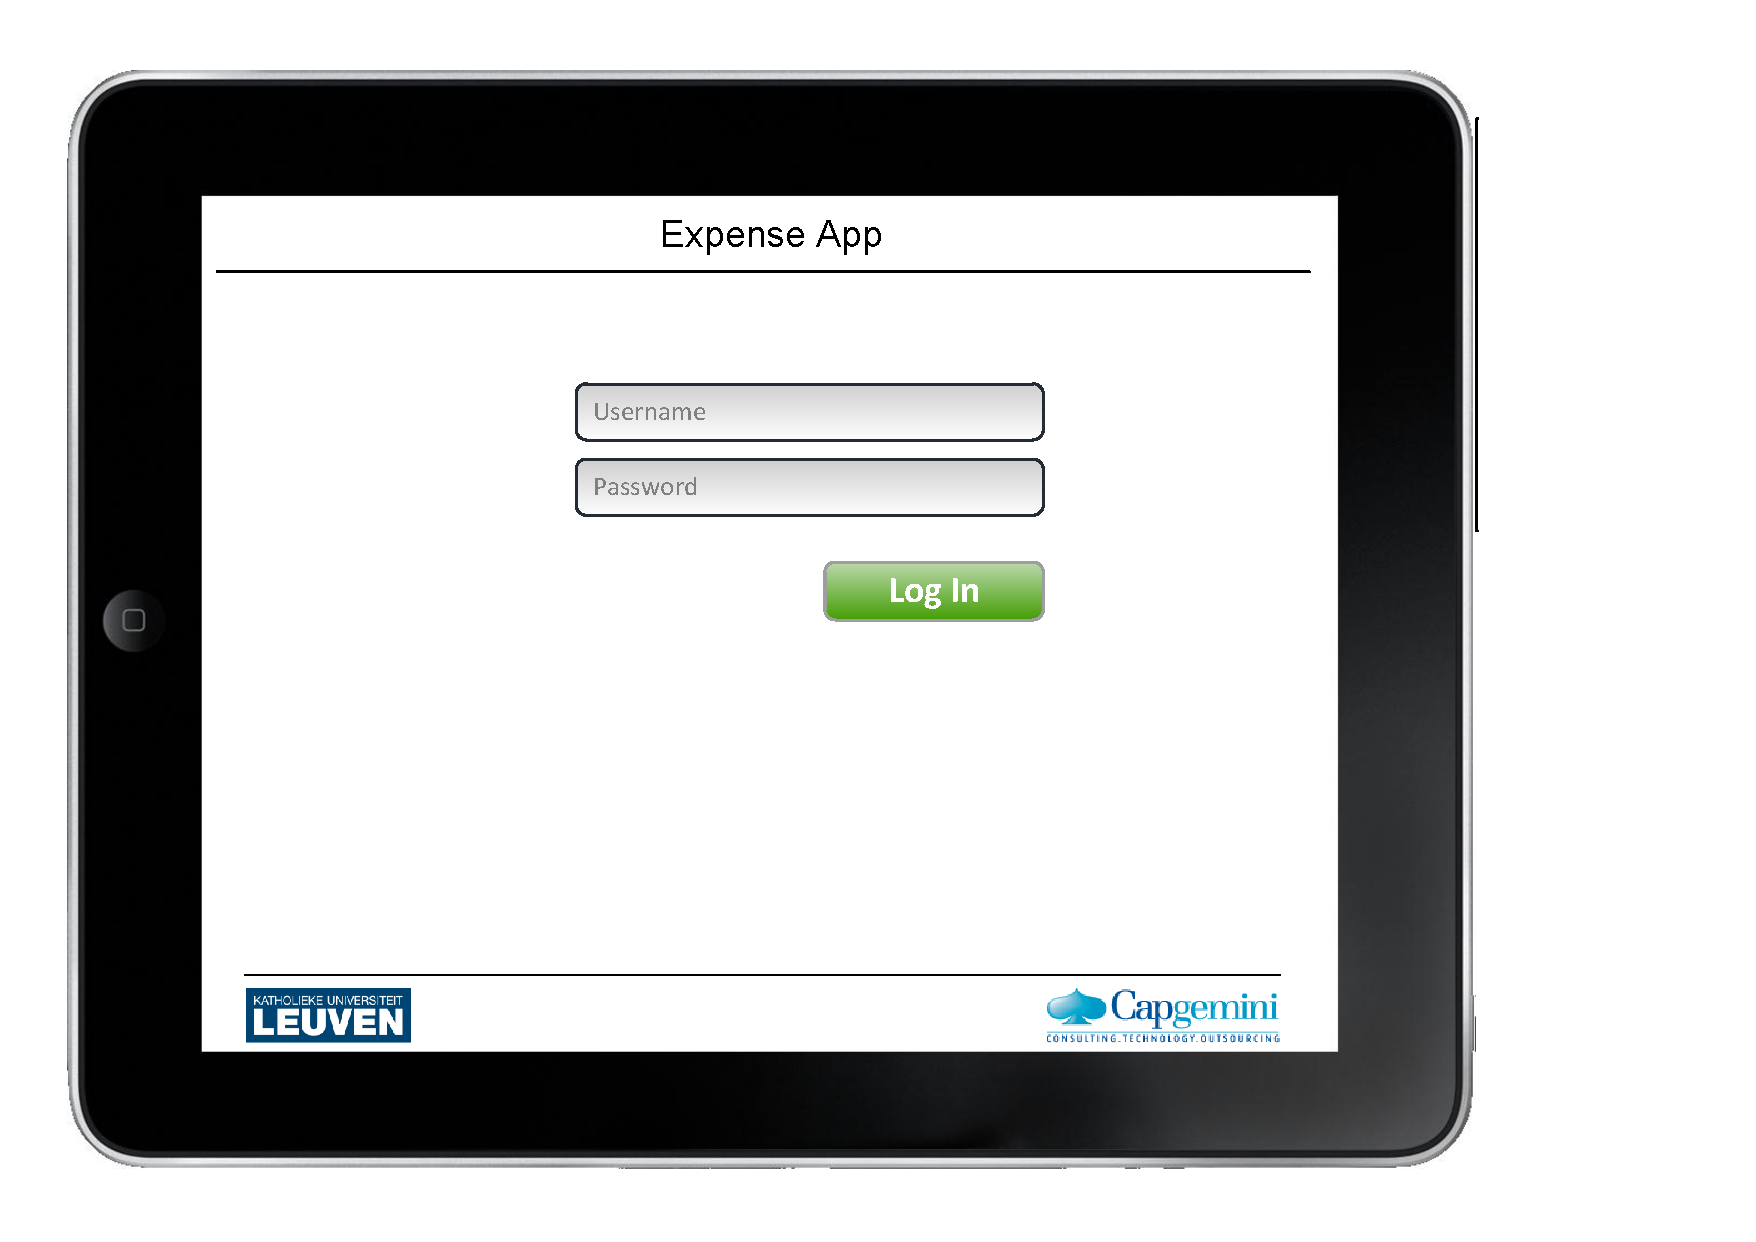
\includegraphics[width=\textwidth]{figs/poc/login-screen.pdf}
    \caption{Login screen}
    \label{fig:app-login-screen}
\end{figure}

\fref{fig:app-login-screen} shows the main screen when the user is not logged in. Use credentials to log in.

Validation: both fields must be filled in, otherwise error.

\subsection{Home screen}

\subsection{Wizard: Step 1 (Your Info)}

\subsection{Wizard: Step 2 (Overview)}

\subsection{Wizard: Step 2 (review expense from abroad)}

\subsection{Wizard: Step 2 (review domestic expense)}

\subsection{Wizard: Step 3 (add expense domestic expense)}

\subsection{Wizard: Step 3 (add expense expense from abroad)}

\subsection{Wizard: Step 4 (Sign \& Send)}

\subsection{Wizard: Validation Dialog}

\subsection{Wizard: Validation element coloring}

\subsection{History}

\subsection{Smartphone version}





%\chapter{The First Appendix}
\label{app:A}


% ... and so on until
%\include{app-n}

\backmatter
% The bibliography comes after the appendices.
% You can replace the standard "abbrv" bibliography style by another one.
\bibliographystyle{apa}
\bibliography{Thesis}

\end{document}